% rubber: watch bkp.glo
% options:
% thesis=B bachelor's thesis
% thesis=M master's thesis
% czech thesis in Czech language
% english thesis in English language

\documentclass[thesis=B,czech]{FITthesis}[2012/05/02]

\usepackage[utf8]{inputenc} % LaTeX source encoded as UTF-8

%\usepackage{biblatex}
\usepackage{graphicx} %graphics files inclusion
% \usepackage{amsmath} %advanced maths
% \usepackage{amssymb} %additional math symbols
\usepackage{listings}

\lstset{ %
  language=Ruby,                % the language of the code
  basicstyle=\ttfamily\small,     % the size of the fonts that are used for the code
  showspaces=false,               % show spaces adding particular underscores
  showstringspaces=false,         % underline spaces within strings
  showtabs=false,                 % show tabs within strings adding particular underscores
  frame=single,                   % adds a frame around the code
  breaklines=true,                % sets automatic line breaking
  breakatwhitespace=true,        % sets if automatic breaks should only happen at whitespace
}

\usepackage{dirtree} %directory tree visualisation
%\usepackage[hyphens]{url}

% % list of acronyms
\usepackage[acronym,nonumberlist,toc,numberedsection=autolabel]{glossaries}
\iflanguage{czech}{\renewcommand*{\acronymname}{Seznam pou{\v z}it{\' y}ch zkratek}}{}
\makeglossaries

\newcommand{\tg}{\mathop{\mathrm{tg}}} %cesky tangens
\newcommand{\cotg}{\mathop{\mathrm{cotg}}} %cesky cotangens

\department{Katedra softwarového inženýrství}
\title{Aplikační podpora pro správu projektů}
\author{Jan Vlnas} %jméno autora bez akademických titulů
\authorWithDegrees{Jan Vlnas} %jméno autora včetně akademických titulů
\supervisor{Ing. Tomáš Kadlec}
\abstractCS{Práce se zabývá modifikací systému \emph{ChiliProject} (navazujícího na systém \emph{Redmine}) prostřednictvím modulů. Porovnává některé open~source webové aplikace pro správu projektů, analyzuje specifika platformy \emph{Ruby on Rails} a zabývá se návrhem, implementací a testováním \emph{rozšíření} existující aplikace bez zásahu do jejího kódu.
Výsledkem práce je několik rozšíření, která mj. decentralizují správu uživatelských rolí a umožňují omezit přístup ke konkrétním zdrojům.
}
\abstractEN{This thesis focuses on modification of \emph{ChiliProject} (forked from \emph{Redmine}) through a set of plug-ins.
The thesis evaluates open~source web applications for project management, analyses some specific aspects of \emph{Ruby on Rails} platform and describes design, implementation, and testing of plug-ins for the existing application.
The resulting plug-ins provide decentralized user roles management, access restriction for particular resources, and more.
}
\placeForDeclarationOfAuthenticity{V~Praze}
\declarationOfAuthenticityOption{4} %volba Prohlášení
\keywordsCS{správa projektů, redmine, chiliproject, ruby, rails, rozšíření, testování}
\keywordsEN{project management, redmine, chiliproject, ruby, rails, plugin, test}

\renewcommand\lstlistingname{Ukázka kódu}
\renewcommand\lstlistlistingname{Ukázky kódu}
\def\appendixautorefname{Příloha}

\widowpenalty=500
\clubpenalty=500

\hyphenation{Chili-Project Red-mine}

\begin{document}

% \newacronym{CVUT}{{\v C}VUT}{{\v C}esk{\' e} vysok{\' e} u{\v c}en{\' i} technick{\' e} v Praze}
% \newacronym{FIT}{FIT}{Fakulta informa{\v c}n{\' i}ch technologi{\' i}}

\newglossaryentry{wiki}{
name=wiki,
description={Systém správy obsahu \citep{WikiWiki}}
} \newglossaryentry{issue tracker}{
name=issue tracker,
description={Systém pro správu úkolů, problémů, požadavků i chyb, viz také \gls{bug tracker}}
} \newglossaryentry{workflow}{
name=workflow,
description={Průběh práce}
} \newglossaryentry{namespace}{
name=namespace,
description={Jmenný prostor}
} \newglossaryentry{SVN}{
name=Subversion,
description={Centralizovaný systém správy kódu}
} \newglossaryentry{git}{
name=Git,
description={Distribuovaný systém správy kódu}
} \newglossaryentry{mercurial}{
name=Mercurial,
description={Distribuovaný systém správy kódu}
} \newglossaryentry{SCM}{
name=SCM,
description={Source Code Management, souhrnné označení software pro správu kódu}
} \newglossaryentry{LDAP}{
name=LDAP,
description={Lightweight Directory Access Protocol, adresářová služba}
} \newglossaryentry{bug tracker}{
name=bug tracker,
description={Systém hlášení úkolů a chyb zpravidla, lze považovat za speciální případ \gls{issue tracker}}
} \newglossaryentry{SaaS}{
name=SaaS,
description={Software as a Service, software poskytovaný formou on-line služby}
} \newglossaryentry{mikroblog}{
name=mikroblog,
description={Zjednodušený a minimalizovaný blog, například Twitter}
} \newglossaryentry{fork}{
name=fork,
description={Odštěpení od hlavní vývojové větve, často s~úmyslem dalšího nezávislého vývoje}
} \newglossaryentry{duck typing}{
name=duck typing,
description={\uv{Pokud to kváká jako kachna, budu tomu říkat kachna} -- není kontrolován typ objektu, postačí že ví, jak odpovědět na zaslan zprávy}
} \newglossaryentry{commit}{
name=commit,
description={Sada změn přidaných do repozitáře kódu}
} \newglossaryentry{submodul}{
name=submodul,
description={V kontextu systému Git: odkaz na externí repozitář z~lokálního repozitáře}
} \newglossaryentry{gem}{
name=gem,
description={V kontextu jazyka Ruby: standardní formát balíčků pro aplikace a knihovny v~Ruby}
} \newglossaryentry{scope}{
name=scope,
description={V kontextu Rails: makro které umožňuje definovat podmínky výběru z~databáze, volání scopes lze řetězit}
} \newglossaryentry{ACL}{
name=ACL,
description={Access Control List, seznam uživatelů a jejich oprávnění pro přístup k~určitému zdroji}
} \newglossaryentry{fixtures}{
name=fixtures,
description={Metoda fixování testovacích dat, viz \autoref{sec:rails_tests}}
} \newglossaryentry{plugin}{
name=rozšíření,
description={Plug-in, zásuvný modul -- kód který rozšiřuje funkčnost aplikace bez potřeby její úpravy}
}
\newglossaryentry{callback}{
name=zpětné volání,
description={Callback -- reference na funkci předaná za účelem jejího dalšího volání; v~Rails se zpětná volání používají k~obsluze událostí}
}
\newglossaryentry{YAML}{
name=YAML,
description={YAML Ain't Markup Language -- textový formát pro serializaci dat, zaměřený na uživatelskou přívětivost; viz \url{http://www.yaml.org/}}
}
\newacronym{ICT}{ICT}{Information and communication technologies}
\newacronym{GPL}{GPL}{GNU General Public License}
\newacronym{AGPL}{AGPL}{Affero General Public License}
\newacronym{DSL}{DSL}{Domain Specific Language}
\newacronym{API}{API}{Application Programming Interface}
\newacronym{MRI}{MRI}{Matz's Ruby Interpreter}
\newacronym{REE}{REE}{Ruby Enterprise Edition}
\newacronym{TDD}{TDD}{Test-Driven Development}
\newacronym{CI}{CI}{Continuous Integration}
\newacronym{HTTP}{HTTP}{Hypertext Transfer Protocol}
\newacronym{SQL}{SQL}{Structured Query Language}
\newacronym{ORM}{ORM}{Object-Relational Mapping}
\newacronym{FIT}{FIT}{Fakultra informačních technologií}

\begin{introduction}

Oddělení \glslink{ICT}{ICT} \glslink{FIT}{Fakulty informačních technologií} má na starost správu softwarového i hardwarového vybavení. Zajišťuje funkčnost fakultních informačních systémů i různých zařízení (tiskárny, počítače v~učebnách). To znamená sledovat a řešit velké množství různých požadavků, od přidání opravy do systému Edux po výměnu toneru v~tiskárnách. Správu požadavků by měl usnadnit jednotný systém pro správu projektů. Takový systém může podporovat i sdílení znalostí (např. v~rámci \gls{wiki}) a správu kódu.

Pro správu projektů oddělení používá systém Redmine\footnote{\url{http://www.redmine.org/}}, který splňuje většinu jejich potřeb. Redmine má však určité nedostatky z~hlediska správy většího množství projektů a uživatelů.

\subsection{Cíl práce}

Cílem práce je zvolit a upravit takový systém, který bude nejlépe vyhovovat potřebám ICT oddělení. Preferované je takové řešení, které bude vyžadovat nejméně zásahů do originálního systému pro zachování kompatibility a udržitelnosti budoucího vývoje systému.

\subsection{Struktura práce}

Text práce je členěn do čtyř kapitol. První kapitola rozebírá současný systém, nakolik jeho funkce odpovídají potřebám ICT oddělení. Druhá kapitola porovnává alternativy k~systému Redmine; zároveň zde odůvodním, proč jsem zvolil přechod na systém ChiliProject. Třetí kapitola řeší některá specifika zvoleného systému a platformy Ruby on Rails. Hlavní část textu tvoří čtvrtá kapitola, kde rozebírám návrh, implementaci a testování jednotlivých úprav. Závěr pak shrnuje výsledky a naznačuje možnosti budoucího vývoje.

\end{introduction}

\chapter{Systém Redmine a požadované vlastnosti}

Při určování požadavků je nutné zohlednit vlastnosti stávajícího
systému, proto nejprve popíšu nejdůležitější vlastnosti Redmine
s~ohledem na funkce vyžadované ICT oddělením.

\section{Popis Redmine}

Redmine je webová aplikace napsaná v~jazyce Ruby s~použitím frameworku
Rails, dostupná pod open~source licencí \gls{GPL} verze 2.

Základem struktury Redmine je \emph{projekt}, ke kterému je možné
přiřadit uživatele. Každý projekt představuje částečně oddělenou
jednotku s~vlastní sadou úkolů, repozitářem kódu a \gls{wiki}.
Specifikem projektů v~Redmine je, že mohou mít hierarchickou strukturu.
Kromě lepší orientace při velkém množství projektů lze tuto hierarchii
využít i pro částečné sdílení některých zdrojů -- například je možné
vypsat úkoly ze všech podprojektů.

Uživatele v~Redmine je možné zařadit do \emph{skupin}. V~rámci projektu
je pak uživateli či skupině přiřazena role (či více rolí), která slouží
pro autorizaci uživatele. Skupiny i role jsou definované globálně,
nicméně rozhodující je, zda má daný uživatel v~projektu členství.

\Gls{issue tracker} představuje systém správy úkolů -- hlášení chyb,
požadavků na změny, návrhy na zlepšení atp. Redmine nabízí několik
možností jak úkoly třídit -- fronty (například chyby, vylepšení) a
kategorie (například podle komponent). Správce však může úkolům
definovat další vlastnosti -- pro jednotlivé projekty je pak možné
zvolit, zda budou mít příslušnou frontu, kategorii či vlastnost
k~dispozici. I~úkoly v~Redmine mohou být hierarchicky uspořádané, navíc na
sebe mohou vzájemně odkazovat -- zde je výhodou, že každý úkol má
v~rámci instance Redmine unikátní číslo, lze proto odkázat na úkol ve
zcela jiném projektu.

Úkoly mají vždy nějaký stav -- například otevřený, vyřešený či
pozastavený. S~tím souvisí podpora \gls{workflow} -- tato funkce
umožňuje určit, jaký stav může určitá role nastavit úkolu s~ohledem na
stávající stav. Například role \emph{vývojář} může změnit úkol, který je
\emph{ve vývoji} na \emph{uzavřený}, nemůže jej však nastavit jako
\emph{nový}.

\Gls{wiki} v~Redmine se příliš neliší od jiných implementací. Jediným
specifikem je, že stránky mohou být uspořádány v~hierarchii -- nejedná
se však o~kompletní podporu \gls{namespace}, jak ji chápe software
MediaWiki\footnote{\url{http://www.mediawiki.org/}} či
DokuWiki\footnote{\url{http://www.dokuwiki.org/}}. Hierarchie má význam
pouze pro navigaci v~rozsáhlejší struktuře stránek.

Redmine, jakožto systém určený především pro správu softwarových
projektů, zahrnuje i \gls{SCM}. Systém podporuje řadu nástrojů pro
správu kódu včetně \gls{SVN}, \gls{git} a \gls{mercurial}. Výhodou této
integrace je propojení kódu s~úkoly -- revize může odkazovat na úkol a
naopak. Zároveň je možné prohlížet zdrojový kód z~webového rozhraní
Redmine a procházet jednotlivé změny.

V~prostředí organizace je důležitá podpora jednotné autentizace
uživatelů -- Redmine standardně podporuje \gls{LDAP}.

Podstatnou vlastností Redmine je i rozšiřitelnost a existence komunity
uživatelů i vývojářů, kteří udržují obrovský systém rozšíření. Redmine
je aktivně vyvíjený od roku 2006 čili lze říci, že se jedná o~software
do jisté míry prověřený časem.

\section{Požadavky}

Požadované vlastnosti jsou tyto:

\begin{itemize}
\item
  issue tracking,
\item
  \gls{SCM},
\item
  hierarchická wiki,
\item
  hierarchická struktura projektů,
\item
  modulární autentizace uživatelů (např. přes \gls{LDAP}),
\item
  podpora uživatelských skupin,
\item
  konfigurovatelná autorizace.
\end{itemize}
Výsledný systém by měl tyto požadavky splňovat, případně by měl nabízet
adekvátní alternativu nebo by chybějící funkce mělo být možné doplnit.

Redmine sice tyto funkce splňuje, některé z~nich mají však určité
nedostatky.

Největší problém představuje \uv{globálnost} -- role a skupiny může definovat
pouze administrátor. Pokud je v~systému větší množství projektů
s~vlastními správci, každý správce může potřebovat jednotnou organizaci
uživatelů ve své hierarchii projektů, stejně tak může vyžadovat roli se
zvláštní sadou oprávnění, která dosud neexistuje. Systém pro správu
projektů by měl usnadňovat organizaci práce, nikoliv práci přidělávat,
proto by měli mít správci projektů možnost definovat skupiny a role
v~rámci svých projektů.

Dalším problémem je viditelnost konkrétních stránek wiki a úkolů. Dejme
tomu že v~rámci jednoho projektu vidí všichni jeho členové všechny
úkoly -- všichni jsou si v~tomto ohledu rovni. Někteří
členové však mohou řešit třebas bezpečnostní problémy,
které by měly být viditelné pouze pro úzkou skupinu uživatelů. Redmine
umožňuje tyto \uv{soukromé záležitosti} řešit pomocí podprojektů --
vytvoří se podprojekt, který bude přístupný pouze vybraným uživatelům.
Není však jisté kdy (a zda vůbec) potřeba privátních úkolů či stránek
nastane, navíc potenciálně každý uživatel může mít zájem vytvořit
privátní úkol -- třeba právě v~případě bezpečnostní chyby, kterou chce
uživatel nahlásit pouze povolaným osobám. Zároveň by však měl mít tento
úkol nadále přístupný, aby byl informován v~případě, že je problém
vyřešen.

Posledním požadavkem, kterým se v~rámci této práce budu zabývat, je
podpora přidávání uživatelů z~\gls{LDAP}. Redmine
pracuje pouze s~lokální databází uživatelů (kromě autentizace) -- uživatel se musí do
systému alespoň jednou přihlásit, aby jej bylo možné přiřadit do
projektu. V~menších organizacích by tento problém byl řešitelný
kompletní synchronizací s~\gls{LDAP}. Adresář Fakulty informačních
technologií však čítá několik tisíc osob, tudíž by se nejednalo o~příliš
schůdné, ani užitečné řešení -- se systémem ICT oddělená potřebuje
pracovat pouze zlomek uživatelů. Jako lepší možnost se nabízí selektivní
přidání uživatele ve chvíli, kdy je s~ním zapotřebí začít pracovat.

Tyto funkce je možné do Redmine doplnit, nicméně jsem nejprve prozkoumal
alternativy -- není vyloučené, že existuje systém, který je funkčně
kompletnější nebo snadněji rozšiřitelný než Redmine.

\chapter{Porovnání alternativních systémů}

Pro správu projektů existuje velké množství aplikací. Některé z~nich
řeší obecnou komunikaci v~týmu se správou úkolů a dokumentů, řada
aplikací má navíc specializované funkce pro správu softwarových
projektů.

Některé nástroje se orientují výhradně na jeden aspekt -- typickým
příkladem je samostatný \gls{bug tracker}\footnote{Například Bugzilla --
  \url{http://www.bugzilla.org/}}, který nabízí pouze správu úkolů, pro
další funkce je nutné použít externí aplikace. Řada takových nástrojů má
unikátní vlastnosti a jejich kombinací lze dosáhnout zajímavých
možností. Nevýhodou je pak samozřejmě roztříštěnost konfigurace a
rozhraní, z~čehož vyplývá náročnější správa a vyšší nároky na uživatele.
V~řadě případů je proto lepší mít jednodušší nástroje, zato dostupné
v~rámci jediného systému.

Pro zúžení výběru jsem stanovil základní kritéria, která každá
posuzovaná aplikace musí splňovat.

\begin{description}
\item[Webová aplikace]
  Ačkoliv distribuované nástroje\footnote{Jako je například Ditz -- \url{http://ditz.rubyforge.org/}} mají své kouzlo,
  nelze po uživatelích vyžadovat instalaci software, aby mohli hlásit
  chyby.
\item[Samostatně hostovaná]
  Software musí být možné provozovat v~rámci
  infrastruktury fakulty, nemůže se jednat o~\gls{SaaS} řešení.
\item[Open~source]
  Aplikaci je možné modifikovat a kompletní zdrojový kód
  je možné zveřejnit.
\item[Aktivní vývoj]
  Poslední vydaná verze by neměla být starší než rok,
  větší komunita uživatelů a vývojářů může být výhodou.
\item[Nezávislost na proprietálních systémech]
  V~rámci integrace do
  fakultní infrastruktury by aplikaci mělo být možné provozovat na
  unixových serverech bez závislosti například na MS SQL Server.
\end{description}
Následující aplikace tato kritéria splňují, posoudil jsem proto jejich
funkčnost a rozšiřitelnost s~ohledem na požadavky.

\section[Trac]{Trac\footnote{\url{http://trac.edgewall.org/}}}

Jeden z~nejpopulárnějších systémů svého druhu; svojí podobou inspiroval
řadu dalších projektů, včetně Redmine \citep{TracRedMine}. Trac je
napsaný v~Pythonu (kompatibilní s~řadou 2.x).

Trac je velice podobný Redmine, zakládá si na menším počtu komponent a
jejich silnější provázanosti. Důraz je kladený především na wiki, jejíž
vlastnosti prostupují celým systémem -- zejména možnost snadno
odkazovat na konkrétní informace v~systému pomocí wiki syntaxe.

Zajímavý je i systém oprávnění, který nerozlišuje mezi skupinami
uživatelů a uživateli samotnými -- uživatelé tak mohou dědit práva od
jiných uživatelů, což nabízí velkou flexibilitu.

Navzdory jednoduchosti systému má výchozí webové rozhraní řadu
nedostatků. Jako největší slabina se jeví navigace -- není zcela jasné,
které odkazy se vztahují ke které komponentě, zda vedou na stránku wiki,
na úkol, nebo třeba na stránku milníku. Tento problém však lze řešit
pomocí alternativních vzhledů a pokročilejší konfigurace.

Nejzásadnější nedostatek systému Trac představuje nemožnost provozovat více
projektů nad stejnou databází. Systém umožňuje poměrně jednoduše
nakonfigurovat nové instance, které sdílí zdrojový kód i uživatele.
Projekty jsou však vzájemně izolované; například není možné jednoduše
odkazovat z~úkolu v~projektu A~na úkol v~projektu B. Není
možné ani vytvářet hierarchii projektů.

Přidání těchto funkcí by znamenalo zásadní zásah do architektury systému
a přepis velké části komponent.

\section[GitLab]{GitLab\footnote{\url{http://gitlabhq.com/}}}

Jedná se o~velice mladý projekt (první verze vyšla v~říjnu 2011)
inspirovaný oblíbenou službou GitHub. GitLab je postavený na frameworku
Ruby on Rails 3.2.

Je vhodný především pro malé vývojářské týmy. Každý projekt
představuje repozitář kódu s~vlastní wiki a úkoly. Mimo to má projekt
k~dispozici i \emph{wall} (nástěnku), kam je možné přidávat soubory, a také
\emph{merge requests} -- užitečná funkce pro revidování nového kódu.

Projekty (potažmo repozitáře) není možné nijak organizovat,
systém oprávnění je příliš jednoduchý a issue tracker velice
minimalistický. Je to však záměrná inspirace GitHubem, který si na
maximální jednoduchosti nástrojů zakládá \citep[snímky
55-71]{Holman2011}.

Logicky je tak GitLab méně vhodný pro velké týmy, velké množství
projektů a nemusí být nejpřívětivější pro netechnické uživatele vzhledem
k~tomu, že klade důraz na přístup ke kódu.

S~ohledem na zaměření i filozofii projektu jsem usoudil, že tento systém
nebude pro potřeby ICT oddělení nejvhodnější. GitLab se však velice
aktivně vyvíjí, tudíž je pravděpodobné, že postupem času bude
představovat stále vitálnější alternativu k~tradičním nástrojům (jako je
právě Redmine). Pro menší týmy se už nyní jedná o~zajímavou volbu.

\section[The Bug Genie]{The Bug Genie\footnote{\url{http://www.thebuggenie.com/}}}

The Bug Genie se profiluje jako nástroj pro agilní vývoj. V~praxi se to
projevuje několika specifickými funkcemi navíc (např. burndown chart),
jinak se jedná o~běžný systém s~issue trackerem a wiki. Implementačním
jazykem je PHP.

Po funkční stránce je systém srovnatelný s~Redmine. Navíc umožňuje
podrobně definovat uživatelské role na úrovni jednotlivých projektů.

Velké množství funkcí však často vede k~horší přehlednosti, a to i přesto, že
The Bug Genie je -- dle oficiální prezentace -- krásný a
(uživatelsky) přívětivý. Z~praktických zkušeností je mi známo, že s~ním měli problém i
zkušenější uživatelé. Některé problémy s~použitelností by šlo vyřešit
zjednodušením kategorizace úkolů, odstraněním přebytečných funkcí a
vylepšením vzhledu, případně zaškolením uživatelů.

Zajímavým způsobem The Bug Genie řeší integraci repozitářů kódu. 
Není zde samostatná komponenta pro procházení repozitáře, ale pracuje
se s~existujícími systémy, jako ViewVC (pro SVN, CVS), gitweb či GitHub.
Uživatel je odkázán na odpovídající stránku v~příslušném systému.
Nevýhodu tohoto řešení představuje správa řízení přístupu ke kódu, protože
nezávislý prohlížeč kódu má samostatně řešená oprávnění. Pravděpodobně
by tak bylo nutné spravovovat autorizaci separátně, nebo ji
synchronizovat mezi více systémy.

Funkce The Bug Genie pokrývají většinu požadavků a zmíněné problémy jsou
řešitelné. Sympatická je i modularita systému, kde i standardně dodávané
funkce jsou řešeny jako nezávislé moduly.

\section[Teambox]{Teambox\footnote{\url{http://teambox.com/}}}

Tato aplikace nemá součásti pro podporu vývoje software, spíše nabízí
řešení pro obecnou spolupráci a komunikaci v~týmu. Přestože autoři
nabízí hostované řešení, zdrojový kód je dostupný pod licencí \gls{AGPL}
verze 3\footnote{\url{https://github.com/teambox/teambox}}. Teambox je
postavený na Ruby on Rails 3.0.

Funkce Teamboxu se točí kolem komunikace mezi spolupracovníky; z~diskuzí
lze vytvořit úkoly a dlouhodobé informace je možné zaznamenat na
\emph{stránkách} (Pages), které však mají ke klasické wiki poměrně
daleko\footnote{Tato funkce je inspirovaná aplikací
  \href{http://backpackit.com/}{Backpack}}.

Teambox je zpočátku velice jednoduchý a přehledný.
S~rostoucími nároky týmu a s~velkým množstvím projektů se situace však rychle mění.
Velké týmy se brzy utopí v~záplavě diskuzí, softwarovým projektům
bude vadit minimalistická správa úkolů a chybějící integrace repozitářů
kódu. Pages není možné hierarchicky třídit a správa oprávnění je velice
omezená.

Pro malé týmy a nesoftwarové projekty však Teambox představuje výborné řešení a
v~současné době se začíná prosazovat i na \glslink{FIT}{FIT}\footnote{\url{http://teambox.fit.cvut.cz/}}.

\section[Open Atrium]{Open Atrium\footnote{\url{http://openatrium.com/}}}

Jedná se o~distribuci systému Drupal (PHP) s~řadou rozšíření pro správu
projektů. Vedle issue trackeru a wiki (Notebook) obsahuje systém i
kalendář, blog (který může plnit funkci diskuzního fóra) a
\gls{mikroblog} (Shoutbox).

Jestli v~něčem Open Atrium skutečně vyniká, tak je to
konfigurovatelnost. Většinu vlastností systému je možné nastavit
z~webového rozhraní -- i mé dosavadní zkušenosti se systémem Drupal
nasvědčují tomu, že krédem vývojářů na této platformě je zřejmě
\uv{configuration over convention}. Síla Drupalu tvoří současně i největší
slabinou systému Open Atrium -- každá pokročilejší úprava obnáší jistý
risk, že se něco rozbije. Konfigurace je však uložená v~databázi, tím
pádem je obtížné sledovat změny a systém se obtížně testuje.

Na samotném Open Atriu je znát jistý \uv{puzzle efekt} dané platformy --
jednotlivé moduly jsou izolované a obtížně propojitelné; například není
možné se odkazovat z~wiki na konkrétní úkol a naopak. Jsou k~dispozici
rozšíření pro Drupal, která tyto problémy řeší. Stejně tak je možná i
integrace procházení repozitáře. Ne všechna rozšíření jsou však
kompatibilní s~Open Atriem a některá se mohou i vzájemně
ovlivňovat.

Teoreticky neexistuje nic, co by se na platformě Drupal / Open Atrium nedalo
postavit. Komplexnost a jistá křehkost celé platformy však činí tento
systém poměrně neatraktivní.

\section[mtrack]{mtrack\footnote{\url{http://mtrack.wezfurlong.org/}}}

mtrack je klonem systému Trac v~jazyce PHP.

I~přes to, že se nejedná o~zcela novou aplikaci (historie sahá do roku
2009), řada funkcí působí poměrně nedotaženým dojmem. Je zde například
jakási koncepce projektů a komponent, avšak kromě jejich administrace se
nezdá, že by s~nimi bylo možné dělat cokoliv jiného -- wiki a issue
tracker sdílejí jediný prostor. Sympatická je správa repozitáře kódu,
na rozdíl od systému Trac je možné přidávat nové repozitáře přes webové
rozhraní a výchozí instalace podporuje, kromě Subversion, také Git a
Mercurial. Wiki je také uložená v~repozitáři, což lze využít k~přímé
editaci dokumentů bez potřeby webového rozhraní.

V~ostatních ohledech se aplikace chová stejně jako Trac, rozdíly jsou
spíše kosmetického charakteru.

Aplikace mtrack má před sebou ještě dlouhou cestu, aby se stala plnohodnotným
řešením, přesto je zde znát jistý potenciál. Pokud se do vývoje zapojí
širší komunita, mohlo by se brzy jednat o~velice atraktivní volbu
v~rámci PHP aplikací.

\section[ChiliProject]{ChiliProject\footnote{\url{https://www.chiliproject.org/}}}

ChiliProject vznikl jako \gls{fork} Redmine
\citep{ChiliProjectWhyFork}. Některé důvody pro odštěpení od Redmine
byly nesystematičnost a uzavřenost vývoje. ChiliProject se proto snaží
být otevřenější (z~hlediska přístupnosti přispěvatelům) a stabilnější
alternativou k~Redmine.

Ačkoliv na první pohled vypadá ChiliProject odlišně, jedná se skutečně
o~pouhé kosmetické rozdíly. Po funkční stránce jsou systémy srovnatelné -- občas
si koneckonců i vyměňují kód. ChiliProject existuje teprve přes
rok, což je v~případě zavedeného a rozsáhlého projektu krátká doba pro
vznik zásadních změn. Je však zřejmé, že oba projekty směřují jiným
směrem; Redmine stále \uv{nabaluje} další funkce a opravy, zatímco
vývojáři ChiliProjectu otevřeně diskutují o~nutnosti radikálních změn
v~kódu. Pomyslné nůžky mezi těmito dvěma projekty se budou nadále
rozevírat.

\section{Zhodnocení}

Z~celkových 23 systémů (\autoref{chap:seznampm}]) jsem jich podrobněji
prozkoumal šest. Nejvíce požadovaných vlastností splňoval systém The Bug
Genie. Usoudil jsem však, že se na tento systém migrovat nevyplatí --
oproti Redmine má z~hlediska webové aplikace velice specifické chování a
strmější křivku učení. Další nevýhodou je použitá platforma -- pominu-li
syntaktické a ideové rozdíly PHP a Ruby (což je spíše otázka osobní
preference), PHP nenabízí srovnatelnou dynamiku, které se věnuji
v~následující kapitole. V~neposlední řadě je
rozdíl v~použitých knihovnách -- Redmine je postavený na Ruby on Rails,
což je časem prověřený a dobře zdokumentovaný framework. The Bug Genie
má vlastní framework, kde prakticky jediným zdrojem informací je
oficiální dokumentace.

Rozhodl jsem se však pro přechod na systém ChiliProject. Struktura databáze
je u~obou systémů -- až na změny v~nejnovějších verzích -- stejná,
migrace z~Redmine tak nepředstavuje žádný problém. Jak jsem již zmínil,
oba systémy se od sebe liší hlavně svým směřováním, ačkoliv
ChiliProjectu chybí jedna z~požadovaných funkcí
(\autoref{sec:private_issues_exist}). Nové verze Redmine vychází
\uv{až když jsou hotové.} ChiliProject má pevně vymezený časový rámec
-- \emph{minor} verze, která je zpětně kompatibilní,
vychází každý měsíc. \emph{Major} verze, která může zahrnovat rozsáhlejší změny,
vychází každý půlrok. V~případě potřeby vyjde \emph{patch} verze (například je nalezena chyba v~zabezpečení).
Pravidelné vydávání nových verzí zajišťuje, že se hotové funkce dostanou
k~uživatelům co nejdříve, vývojáři zase mají jasně vymezený časový
rámec, ve kterém mohou pracovat. Je to podobný model, byť zjednodušený,
jaký používá například Linux a Mozilla Firefox
\citep{MozillaDevProcess}.

\chapter{Analýza platformy}
\label{chap:analyza_navrh}

Pro implementaci úprav systému je nutné zvážit specifické vlastnosti
platformy, na které je systém postavený. V~této kapitole proberu některé
charakteristiky platformy používané systémem ChiliProject, které určí
formu výsledné práce.

\section{Vlastnosti platformy}

ChiliProject používá framework Ruby on Rails ve verzi 2.3.

Samotný jazyk Ruby má řadu specifických vlastností, které značně
rozšiřují možnosti implementace. Zaměřím se proto na některé dynamické
vlastnosti jazyka Ruby, základy architektury Ruby on Rails aplikace,
systém rozšíření a strukturu testování.

\subsection{Dynamické vlastnosti jazyka Ruby}
\label{sec:vlastnosti-ruby}

Ruby je dynamický, silně typovaný\footnote{Přesněji řečeno používá
  \gls{duck typing}, na rozdíl od slabě typovaných dynamických jazyků,
  jako je JavaScript či PHP, však Ruby neprovádí implicitní konverzi typů
  \citep{Lamontagne2007}} jazyk, inspirovaný vlastnostmi jazyka
Smalltalk a syntaxí jazyka Perl \citep{Stewart2001} -- ačkoliv podle
autora Ruby, Yukihiro \uv{Matz} Matsumoto, podobu jazyka ovlivnil i editor
Emacs \citep{Matsumoto2012}.

V~oblasti současných dynamických programovacích jazyků představuje Ruby do jisté
míry extrém. Prakticky jakoukoliv vlastnost programu je možné zkoumat
a měnit \uv{za běhu}, se všemi pozitivy i negativy, která z~toho vyplývají.
Zpravidla to bývá využíváno k~metaprogramování \citep[3c]{why2008}.
Framework Rails využívá metaprogramování mj. v~podobě maker, která se
hojně využívají u~modelů, např. pro validaci atributů a definici
asociací.

S~dynamičností Ruby souvisí i otevřenost tříd a možnost redefinice
metod, tzv. monkey patching \citep[str. 293]{Olsen2011}. Každá třída
může být opět otevřena a doplněna o~další metody, případně existující
metody mohou být zcela nahrazeny. Metody mohou být přidávány a měněny
také vložením modulů (v~tomto kontextu nazývanými mixins); Ruby tímto
nahrazuje vícenásobnou dědičnost (multiple inheritance). Moduly však
mohou být do třídy vloženy i zvenčí.

Pro představu uvedu ukázku. Mějme definovanou třídu Example
s~metodou hello:

\begin{lstlisting}
class Example
  def hello
    "Hello"
  end
end
>> puts Example.new.hello #=> "Hello"
\end{lstlisting}
Nyní vytvoříme patch pro tuto třídu:

\begin{lstlisting}
module ExamplePatch
  def greeting
    "Odelay!"
  end
end
\end{lstlisting}
Původní třídu rozšíříme o~tento modul:

\begin{lstlisting}
>> Example.send :include, ExamplePatch
>> puts Example.new.greeting #=> "Odelay!"
\end{lstlisting}
Pro redefinici existujících metod z~modulu je vhodné použít makro \\
\lstinline!alias_method_chain! z~knihovny
ActiveSupport (která je součástí Rails).

\begin{lstlisting}
module ExamplePatch
  def self.included(base)
    base.class_eval do
      alias_method_chain :hello, :patch
    end
  end

  def hello_with_patch
    hello_without_patch + " world!"
  end
end

>> Example.send :include, ExamplePatch
>> puts Example.new.hello #=> "Hello world!"
\end{lstlisting}
Toto makro zaručí, že interpret najde upravenou metodu a současně umožní
zavolat původní metodu. Několik modulů tak může přepsat tutéž metodu a
volání zřetězit.

Popsané vlastnosti Ruby dávají rozšířením mnoho možností jak pozměnit jádro
aplikace bez potřeby zásahu do originálního kódu. Díky tomu je možné
vůbec uvažovat o~implementaci úprav v~rámci rozšíření bez potřeby
odštěpení od originální aplikace.

\subsection{Architektura Ruby on Rails}

Framework Rails má zajisté velký podíl na popularizaci jazyka Ruby i
architektury Model--view--controller (MVC) pro webové aplikace. Jak
poukazuje \citep{Krzywda2011}, ve skutečnosti má MVC v~pojetí Rails
blíže k~paradigmatu Model 2, který vznikl s~ohledem na specifika
webových aplikací \citep{McCallister2004}. Označení MVC používá řada
webových frameworků inspirovaných Rails (zejména v~PHP), nicméně
rozlišení oproti architektuře Model 2 (někdy se hovoří o~\emph{MVC2}) a
klasickému MVC nabývá na významu s~popularizací klientských frameworků
(jako například Backbone.js nebo Ember.js), které mají k~původnímu
návrhu MVC blíže.

Ruby on Rails, jakožto \uv{opinionated} framework \citep[kpt. 4, Make
Opinionated Software]{Fried2009}
předpokládá totožnou MVC strukturu u~všech aplikací. ChiliProject
v~tomto směru není výjimkou, jádro aplikace je rozdělené do těchto tří vrstev:

\begin{description}
\item[Model] \hfill \\
Představuje doménovou logiku (business logic), aplikace a v~případě Rails i zdroj dat. \hfill \\
Většinou se mapuje na odpovídající tabulku v~databázi.
\item[Controller] \hfill \\
Propojuje pohled a model. \hfill \\
Zpracovává přijatá data a připravuje data pro šablony. \hfill \\
Jednotlivé veřejné (public) metody controlleru představují akce. \hfill \\
V~této vrstvě se většinou řeší autorizace.
\item[View (pohled)] \hfill \\
Prezentuje data z~controlleru. \hfill \\
Většina akcí controlleru má svůj pohled, současně tyto pohledu mohou pracovat s~dílčími (partial) pohledy
\end{description}

Vedle toho zde existují tzv. helpers, což jsou pomocné funkce, které
mohou sloužit ke sdílení funkcionality v~pohledech.

Jedno z~často opakovaných pravidel při vývoji Ruby on Rails aplikací je
\uv{Skinny controller; fat model}\citep{Buck2006} -- controller by měl
obstarávat pouze jednoduché dotazování a přípravu dat. Většina logiky --
ať už složitější dotazy nebo určité zpracování a reprezentace dat -- by
měla být obstarána v~modelu, čímž se redukuje duplikace kódu. Bohužel,
důsledné následování tohoto pravidla vede k~jinému extrému -- model bude mít
příliš mnoho funkcí bez zjevné souvislosti \citep{Libbery2011}.
ChiliProject tímto problémem místy trpí; rozdělení modelů na logicky
související celky \citep{Grimm2012} by mohlo být předmětem refaktorování
v~budoucích verzích.

\subsubsection{ActiveRecord}

Pro objektově relační mapování (ORM) používá Rails knihovnu
ActiveRecord, která implementuje stejnojmenný návrhový vzor \citep[str.
160]{Fowler2003}. Důsledkem je, že jak perzistence, tak doménová logika
aplikace je součástí modelů. ActiveRecord v~Rails, v~souladu
s~paradigmatem \uv{convention over configuration} však předpokládá, že
databáze bude splňovat specifické konvence pojmenování tabulek a
sloupců. Tím pádem není ve většině případů nutné řešit mapování mezi
databází a objekty. Samozřejmě má tento přístup svá úskalí: u~nové
aplikace od začátku vyvíjené pro Rails je to výhoda, v~případě
kompatibility s~existující databází postavené na odlišných konvencích je
to problém -- pro takové případy však není ActiveRecord vhodné ani
doporučené používat.

Konvence pojmenování v~ActiveRecord jsou následující:
\begin{itemize}
\item Název modelu je v~singuláru (\lstinline!Project!), název odpovídající tabulky
v~plurálu (\lstinline!projects!).
\item Primární klíč záznamu je ve sloupci \lstinline!id!, ActiveRecord nepředpokládá používání přirozených
klíčů.
\item Sloupce cizích klíčů mají název ve tvaru \lstinline!model_id!,
např. \lstinline!project_id!.
\item Některé názvy sloupců jsou rezervované pro ActiveRecord, především se jedná o~sloupec \lstinline!type!
používaný pro dědění v~rámci jedné tabulky (Single Table Inheritance
\citep[str. 278]{Fowler2003})
\end{itemize}

Většinu těchto konvencí lze u~jednotlivých modelů změnit, v~praxi je
však jednodušší přizpůsobit se. ChiliProject tato pravidla také ve
většině případů dodržuje.

Změny v~databázi jsou řešené prostřednictvím migrací, což jsou krátké
skripty, které provádí dílčí změny v~databázi -- přidávání / odebírání
tabulek a sloupců, mohou také měnit existující záznamy. Migrace se
provádí v~pořadí, ve kterém byly vytvořeny. Každá má dvě metody:
\lstinline!up! a \lstinline!down!, což je de facto dopředný a zpětný
chod. Pokud migrace v~metodě \lstinline!up! vytvoří tabulku, metoda
\lstinline!down! tutéž tabulku smaže. Rails od verze 3 umí k~některým
takovým změnám automaticky přiřadit opačný postup, potom si migrace
vystačí s~jedinou metodou \lstinline!change!.

Charakteristické pro Rails je, že databázi považuje jen za \uv{hloupé}
úložiště dat. Ačkoliv je možné v~migraci definovat některá omezení a unikátní klíče,
Rails vyžaduje provádění kontroly dat na aplikační úrovni.
ActiveRecord sám o~sobě neřeší ani referenční integritu či
kompozitní klíče; jsou-li však takové funkce vyžadovány, v~řadě případů
je doplní rozšíření. Případně lze ActiveRecord zcela nahradit jiným ORM
frameworkem jako je například DataMapper nebo řada specializovaných
knihoven pro nerelační databáze -- například MongoMapper. ActiveRecord
se zkrátka nesnaží být \uv{stříbrnou kulkou} pro všechny případy.

\subsection{Struktura rozšíření, Rails Engines}

ChiliProject používá systém Engines, který umožňuje rozšířit
funkce aplikace prostřednictvím dílčích \uv{miniaplikací} -- každý
engine může mít vlastní modely, pohledy a controllery, které jsou
v~běžící aplikaci integrovány do jediného celku s~vlastními komponentami
aplikace. Engines je standardní součást Ruby on Rails od verze 3.1.
Z~toho důvodu už původní modul není vyvíjený, nicméně ChiliProject jej
využívá z~důvodu kompatibility s~Rails 2.3.

Protože pouhé přidávání komponent však zpravidla nestačí, může rozšíření
upravovat existující metody (viz
\ref{sec:vlastnosti-ruby}) a
nahrazovat výchozí pohledy -- zde však samozřejmě nastává problém, pokud
více rozšíření potřebuje nahradit stejný pohled. Proto má ChiliProject
systém zpětných volání, tzv. hooks\footnote{\url{http://www.redmine.org/projects/redmine/wiki/Hooks}}.
Ty se většinou volají z~pohledů, ale v~ojedinělých případech jsou
použity i v~controlleru či v~modelu.

Vedle toho mají rozšíření k~dispozici standardní mechanismy zpětných volání.
Například filtry v~controlleru, které se
zavolají před provedením akce\footnote{Eventuálně po provedení či v~obou
  případech,
  \url{http://apidock.com/rails/v2.3.8/ActionController/Filters/ClassMethods}}. Ty se
často používají pro autorizaci přístupu a k~načtení dat pro
pohled. Obdobný systém existuje i pro modely, rozšíření se může nechat
zavolat například po vytvoření nového záznamu, uložení změn či před
validací\footnote{\url{http://apidock.com/rails/v2.3.8/ActiveRecord/Callbacks}}.

Celkově je na systému rozšíření pro ChiliProject zajímavé, jak málo
funkcí řeší samotná aplikace. Většinu potřeb rozšíření obstará samotné
Ruby ve spolupráci s~Rails. Je to příjemný rozdíl například oproti PHP,
kde řada aplikací spoléhá čistě na explicitní systém událostí
a zpětných volání -- pokud událost není vyvolána na správném místě, jedinou možností je
většinou zásah do jádra aplikace.

\subsection{Struktura testů}
\label{sec:rails_tests}

Jak už jsem dříve naznačil, Ruby je dynamický jazyk ad absurdum.
U~složitějších aplikací je prakticky nemožné odhadnout, jak se budou chovat
-- nemalá část logiky vzniká až za běhu programu. I~to
je zřejmě jeden z~důvodů, proč komunita Ruby investuje nemalé úsilí do
testování kódu; není zde žádný překladač, který mnohdy odchytí nejhrubější chyby
v~logice programu. Jedinou zárukou funkčnosti programu je jeho úspěšný běh.
Ve skutečnosti každý vývojář testuje svou aplikaci, byť manuálně.
Automatizované testy vypadají jako zbytečná práce navíc, s~narůstající
komplexitou aplikace se však začne rychle vyplácet \citep{Rappin2011}.

Ruby on Rails pro testování standardně používají framework Test::Unit,
který patří do rodiny xUnit frameworků \citep{FowlerXunit}. Každá třída
v~aplikaci má odpovídající test case. Metody test case se nazývají
testy. V~rámci testů se porovnává očekávaný stav s~reálným chováním
aplikace pomocí různých \lstinline!assert! metod (assertions). Pokud
\lstinline!assert! selže (např. nějaká metoda vrátí \lstinline!false!
namísto očekávaného \lstinline!true!), test neprošel.

Rails řadí testy do několika kategorií -- zjednodušeně lze říct, že
kategorizace je dána typem testované třídy.

\begin{itemize}
\item
  Jednotkové (unit) testy slouží pro testování modelů a helperů.
\item
  Funkcionální (functional) testy slouží pro testování controllerů a
  případně pohledů.
\item
  Integrační (integration) testy prověřují aplikaci jako celek tím, že
  simulují chování uživatele.
\end{itemize}
Vedle toho někteří vývojáři pracují s~akceptačními (acceptance) testy,
které by měly ověřit, zda funkčnost aplikace vyhovuje požadavkům
zadavatele. Zde se často používá framework Cucumber\footnote{\url{http://cukes.info/}};
chování aplikace se popisuje v~rámci tzv. features, kde jsou jednotlivé
scénáře rozepsány v~jazyce Gherkin -- ten záměrně vypadá jako přirozený
jazyk, ačkoliv se jedná o~\gls{DSL}. Záměr je takový, že specifikace pro
Cucumber je čitelná i pro netechnického uživatele, což by mělo usnadnit
komunikaci s~klientem. Jak však poukazuje \citep{Kinsella2011}, v~praxi
tato idea příliš nefunguje -- výsledkem jsou často \uv{integrační testy
v~přestrojení,} zbytečně dlouhé, hůře strukturované, a přesto pro
klienta nečitelné.

ChiliProject používá Test::Unit v~kombinaci s~knihovnou
Shoulda\footnote{\url{https://github.com/thoughtbot/shoulda}}. Ta
zahrnuje dvě funkce: jednak přidává další užitečné \lstinline!assert!
metody, jednak přidává podporu pro kontext -- ten umožňuje sdílení stavu
mezi jednotlivými testy. Zatímco Test::Unit umožňuje připravit sdílený
stav mezi všemi testy v~rámci jednoho test case pomocí metody
\lstinline!setup!, kontext umožňuje test case dále rozčlenit do menších
částí, jenž mají svůj vlastní stav a neovlivňují ostatní testy. Výhodou je,
že jednotlivé testy mohou být kratší, a tím pádem je snazší
identifikovat problematické chování. Kromě toho Shoulda nahrazuje metody
test popisnějším makrem \lstinline!should!. Pro praktický příklad viz \autoref{lst:shoulda}.

\begin{lstlisting}[float,caption={Test case s~frameworky Test::Unit a Shoulda},label=lst:shoulda]
class UserTest < ActiveSupport::TestCase
  # Metoda setup je sdilena pro vsechny testy
  # v~tomto test case
  def setup
    @user = User.generate!
  end

  should "be a user" do
    assert @user.kind_of?(User)
  end

  context "administrator" do
    # Makro setup se provadi jen pro testy
    # v~tomto kontextu
    setup do
      @user.is_admin = true
    end

    # Konkretni test
    should "be allowed to do anything" do
      assert @user.allowed_to?(:anything)
    end
  end

end
\end{lstlisting}

Testy musí mít k~dispozici data, na kterých bude prověřována
funkčnost aplikace. Rails standardně podporují tzv. fixtures, což jsou
serializovaná data (nejčastěji ve formátu \gls{YAML}, jenž je činní
snadno editovatelnými), která jsou před provedením testů načtena do
databáze. Fixtures musí být průběžně udržovány a s~rostoucí komplexností
aplikace se komplikuje i jejich struktura. Proto se místo toho většinou
používají generátory dat (data factories), které vytvoří požadované
objekty -- včetně závislostí -- až když jsou zapotřebí. ChiliProject
používá oba přístupy, pro generování dat používá knihovnu
ObjectDaddy\footnote{\url{https://github.com/edavis10/object_daddy}}.

Další technikou, byť v~ChiliProjectu ne příliš používanou, jsou tzv.
mock objekty. S~tím často souvisí i tzv. stubs, pro podrobnosti viz
\citep{FowlerMocks}. Mock objekty i stubs umožňují vytvořit
\uv{testovacího náhradníka} (test double) objektu, což je užitečné
v~případech, kdy použití skutečného objektu je příliš náročné nebo přímo
nemožné (například při práci s~externím API). Kromě toho je pro
mock objekty možné určit, kolikrát má být zavolána určitá metoda a
s~jakými parametry -- pokud předpoklad není splněný, test selže. Ačkoliv
Ruby činní nasazení mock objektů velice jednoduché, jejich přílišné
používání může vést k~zavádějícím a mnohdy i špatně udržovatelným testům
\citep{Parsons2011}.

Na sadě testů pro ChiliProject je zřejmé, že se již dlouho vyvíjí
společně s~aplikací, nicméně už samotná existence a funkčnost testů je
nesmírně důležitá. Představuje konvenci na které mohou stavět testy
jednotlivých rozšíření. Zároveň je možné testovat integraci rozšíření,
zda jejich nasazení nenaruší standardní funkce systému.

Ožehavá otázka: \uv{Co všechno testovat?} Obligátní odpověď \uv{všechno}
v~praxi neobstojí a ani by to neměl být hlavní cíl testů. Jak podotýká
D.H.H. \citep{HanssonTestingTSA}, testy představují kód, který se
také musí udržovat, jinými slovy: nejsou zadarmo. Cílem by nemělo být
100\% pokrytí kódu a rozhodně by psaní testů nemělo zabírat více času
než psaní samotné aplikace. Z~hlediska dlouhodobé udržitelnosti je lepší
mít malou a nekompletní, zato funkční a přehlednou sadu testů, ve které
se nový vývojář snadno zorientuje. Testy jsou doplňovány s~nalezenými
chybami, což zmenší riziko regresí. Naopak, i pokud je poměr testů vůči
samotné aplikaci 3:1, není to zárukou bezchybnosti.

\section{Možnosti implementace funkcí}

Požadované funkce mohou být implementované dvěma způsoby: úpravou
samotné aplikace ChiliProject nebo v~rámci individuálních rozšíření.
Tyto možnosti se vzájemně nevylučují, do jádra by mohly být přidané
pouze některé funkce, i tak by ale tato cesta měla jisté následky.

Modifikace jádra představuje odštěpení od hlavní vývojové větve,
\gls{fork}. Je nutné sledovat změny v~originální aplikaci a hrozí, že
dojde ke konfliktům mezi forkem a originální aplikací. Integrované
funkce je obtížné vzájemně odlišit a vyextrahovat v~případě, že by byla
zapotřebí pouze jejich část. Výhodou je naopak potenciálně \uv{čistší}
implementace změn s~menší duplikací kódu.

Naproti tomu rozšíření se vždy nasazují na oficiální verzi aplikace.
Každé z~nich představuje ohraničenou sadu funkcí, snadno přenositelné a
snadno odstranitelné. To má i velkou výhodu pro udržitelnost --
individuální rozšíření je velice přístupné pro externí přispěvatele,
kteří mohou objevit chyby a doplnit další funkce. Fork upravený pro
potřeby konkrétní organizace je interní řešení, za jehož osud zcela
odpovídá daná organizace.

Mým cílem bylo veškeré požadované funkce implementovat jako rozšíření --
jak jsem již rozebral, jsou to především vlastnosti jazyka Ruby, které
umožnily tohoto cíle dosáhnout. Jen v~jediném případě jsem se nevyhnul
zásahu do originální aplikace, podrobněji viz
\ref{sec:oprava-engines}.

\section{Cílové verze prostředí}

Prvotním předpokladem implementace byla kompatibilita s~poslední verzí
oficiálního interpreta Ruby, \gls{MRI} 1.9.3. Samotný ChiliProject
podporuje také verze 1.8.7 a 1.9.2, avšak pokud je to možné, nevyplatí se
je používat i proto, že oproti novější verzi poskytují horší výkon. Je tomu
tak i v~případě \gls{REE} \citep[End of Life]{REEEOL}. S~ohledem na stáří
knihoven používaných v~systému ChiliProject zpravidla ani není problém
zajistit kompatibilitu se staršími verzemi interpretu -- stále větší
výzvou však bude udržovat krok s~novými verzemi Ruby.

Rozšíření byla testovaná s~vývojovou verzí ChiliProject 3.2.0,
pravděpodobně by však s~menšími úpravami mohla být kompatibilní jak se
staršími verzemi, tak se systémem Redmine.

\chapter{Návrh a implementace rozšíření}

Na základě analýzy požadavků lze určit rozložení požadovaných
funkcí do samostatných rozšíření. Samozřejmě by bylo možné modifikace
seskupit do jediného celku -- to by sice snížilo duplikaci některých částí kódu,
ale výsledek by byl nepřehledný a obtížně udržovatelný. Proto jsem funkce
rozdělil do dílčích částí tak, aby každé rozšíření bylo použitelné
nezávisle na ostatních; sdílené či vzájemně se překrývající části kódu
mohou být vyjmuté do samostatného rozšíření.

\begin{enumerate}
\item Správa uživatelských skupin na úrovni projektů (\ref{sec:project_group});
\item správa rolí na úrovni projektů, úzce souvisí i s~\gls{workflow}, výsledné rozšíření zahrnuje i
správu workflow pro role na úrovni projektů (\ref{sec:project_roles});
\item wiki stránky s~omezeným přístupem (\ref{sec:private_wiki});
\item úkoly s~omezeným přístupem (\ref{sec:private_issues});
\item přidávání uživatelů z~\gls{LDAP} (\ref{sec:add_ldap_users}).
\end{enumerate}

Tato rozšíření jsem zahrnul do hlavního repozitáře
\emph{chiliproject-fit} společně s~aplikací ChiliProject, lehce
přizpůsobenou pro testování (nejedná se však o~funkční zásahy do jádra)

Každé rozšíření pracuje s~odlišnými částmi systému ChiliProject, proto
se návrhu a implementaci věnuji pro každé rozšíření zvlášť. Některé
základní postupy přitom zůstávají pro každé rozšíření stejné.

\section{Příprava testovacího prostředí}

Psaní testů pro rozšíření bohužel není příliš časté, ačkoliv to
ChiliProject přímo podporuje. Informace v~této oblasti jsou poměrně
střídmé a narazil jsem na problémy s~provozováním testů pod Ruby 1.9.3
-- zřejmě se nikdo nepokoušel testovat rozšíření pod touto verzí.

Prvním krokem tedy bylo \uv{otestovat testovací prostředí} a zajistit
jeho stabilitu. Po vzoru metodiky \gls{TDD} je tak možné psát testy
současně s~funkčním kódem. Zároveň je v~průběhu vývoje možné využívat
\gls{CI}.

Protože veškerý kód v~této práci je pod open~source licencemi,
je od začátku hostovaný ve veřejných repozitářích na serveru GitHub.
Není to pouze otázka osobní preference, existuje řada nezávislých služeb,
které nabízí projektům na GitHubu užitečné funkce navíc. Konkrétně
v~tomto případě jsem se rozhodl využít službu Travis-CI\footnote{\url{http://travis-ci.org/}},
která poskytuje hostované řešení \gls{CI} pro open~source projekty zcela zdarma.

Travis-CI funguje následovně: ze serveru GitHub dostane oznámení, že v~cílovém
repozitáři přibyl nový \gls{commit} (přes tzv. post-commit hook). Travis
spustí \emph{build}: vytvoří virtuální stroj, stáhne do něj repozitář
s~kódem, nainstaluje potřebné knihovny a spustí sadu testů. Ty typicky
vrací návratový kód -- jak je zvykem v~Unixu: \lstinline!0! znamená
úspěch, jiné číslo neúspěch. Travis kontroluje tento návratový kód a
podle toho označí build jako úspěšný či neúspěšný. Průběh buildu je
možné sledovat v~reálném čase přes webové rozhraní.

Použití \gls{CI} má několik výhod. Je zde jednodušší provádět časově
náročné testy (provedení celé testovací sady ChiliProjectu trvá 15
minut!) Také je jednodušší kombinovat různé vlastnosti
prostředí; testy lze provádět například s~různými databázovými systémy
či jinými verzemi Ruby -- kombinací těchto variant vznikne matice, tzv.
\emph{build matrix}. Má-li aplikace podporovat tři různé databázové systémy
a tři verze interpreta, představuje to devět různých buildů -- testovat
něco manuálně by bylo přinejmenším obtížné. Hostovaná služba je pak
samozřejmě výhodná, neboť vyžaduje minimální konfiguraci -- do
repozitáře zpravidla stačí přidat konfigurační soubor a aktivovat
post-commit hook. Výsledek buildu je veřejně přístupný, může tak sloužit
jako základní indikátor pro vývojáře i uživatele, zda je aktuální
vývojová verze aplikace použitelná.

Travis-CI jsem použil pro dva případy: testování ChiliProjectu jako
celku s~instalovanými rozšířeními a testování jednotlivých
rozšíření.

První případ představoval přidání konfigurace pro Travis-CI do
repozitáře \emph{chiliproject-fit}. Každé přidané rozšíření je
\gls{submodul} pro Git, proto je nutné před testem provést jejich
inicializaci. Současně je nutné připravit testovací databázi --
poskytnout údaje pro připojení, databázi vytvořit a spustit migrace. Ve
výsledku se de facto jedná o~integrační test -- v~systému jsou zavedená
všechna rozšíření a úspěšné provedení testů je minimální zárukou toho,
že žádné z~nich nenarušilo funkce systému.

Druhý případ je složitější -- rozšíření bez aplikace, kterou rozšiřuje,
nelze spustit, natož testovat. Tento problém řešili vývojáři systému
Radiant \citep{Muhl2012}. Před testováním se provede skript, který
stáhne samotnou aplikaci a přesune do ní (již stažené) rozšíření. Skript
jsem přizpůsobil pro ChiliProject a zobecnil jsem jej tak, aby byl snadněji
konfigurovatelný pro další rozšíření. Kostrou tohoto řešení je rozšíření
\lstinline!chiliproject_test_plugin! které posloužilo jako prototyp
k~odladění.

Při prvních testech reálných rozšíření jsem však narazil na záhadný
problém.

\section{Oprava Engines}
\label{sec:oprava-engines}

Rozšíření pro ChiliProject jsou postavená na modulu Engines a
využívají jej i testy. Rozšíření zpravidla používá
\gls{fixtures} originální aplikace, zároveň může soubory fixtures
přidávat nebo i nahrazovat. Engines to řeší tak, že postupně zkopíruje
soubory z~původní aplikace a z~rozšíření do dočasného adresáře, cestu
k~němu pak přidá na začátek globální proměnné
\lstinline!$LOAD_PATH!. To zaručí, že se fixtures načtou z tohoto
adresáře.

V~Ruby 1.9 se však změnila specifikace standardní funkce pro vytvoření
adresáře \lstinline!FileUtils.mkdir_p! -- původně vracela řetězec, nyní
vrací pole. Engines (v~modulu \lstinline!Engines::Testing!) přidávají
výstup této funkce bez další kontroly do proměnné \lstinline!$LOAD_PATH!
-- pod Ruby 1.9 se tak v této proměnné ocitne pole, což zcela zmate
systém načítání závislostí. Volání funkce \lstinline!require! (pro
načtení souboru) pak způsobí pád testů.

Oprava této chyby byla poměrně banální, největším problémem bylo ji
nalézt a otestovat -- testy Engines jsou pod Ruby 1.9 zcela nefunkční.
Výsledkem je opravený \gls{fork} modulu \lstinline!engines!, který jsem
zahrnul do distribuce \emph{chiliproject-fit}. Problém byl
nahlášený vývojářům ChiliProject, bohužel oprava dosud nebyla zahrnuta
do oficiální verze\footnote{\url{https://www.chiliproject.org/issues/952}}.

S~funkčním testovacím prostředí už bylo možné začít implementovat
jednotlivá rozšíření.

\section[Správa uživatelských skupin na úrovni projektů]{Správa uživatelských skupin na úrovni projektů (ChiliProject
Project Group)}
\label{sec:project_group}

\subsection{Specifikace}

Cílem tohoto rozšíření je decentralizovat správu uživatelských skupin
tak, aby se jejich vytváření a modifikace obešla bez zásahu
administrátora. Jako nejvhodnější možnost se nabízí navázání skupin na
projekt, kde už s~nimi bude moct pracovat správce projektu.

Správce projektu s~oprávněním pro modifikaci projektových skupin může:

\begin{enumerate}[1.]
\item
  Vytvořit novou či smazat existující projektovou skupinu,
\item
  přidat a odebrat členy projektové skupiny,
\item
  změnit název skupiny
\end{enumerate}
Správce projektu s~oprávněním pro správu členů projektu může:

\begin{enumerate}[1.]
\setcounter{enumi}{3}
\item
  Přiřadit skupině roli v~projektu; příslušnou roli dostanou všichni
  členové skupiny.
\end{enumerate}
Projektové skupiny jsou k~dispozici všem podprojektům (lze jim přiřadit
roli -- požadavek 4), nelze je ale v~rámci podprojektu modifikovat
(požadavky 1 až 3).

Nadále bude možné používat i standardní funkci globálních skupin, které
jsou k~dispozici všem projektům a může je modifikovat pouze
administrátor.

\subsection{Existující řešení}

Některé z~požadavků částečně splňuje rozšíření Group Assignee\footnote{\url{http://www.redmine.org/plugins/groupsassignee}},
které umožňuje přiřadit skupině zodpovědné osoby, jenž mohou přiřazovat a
odebírat členy. Ačkoli to částečně řeší decentralizaci správy, stále je
nutné, aby administrátor skupiny nadefinoval. Navíc všechny skupiny stále
existují v~globálním kontextu, což při jejich větším množství vede
k~nepřehlednosti.

\subsection{Systém uživatelů, skupin a rolí}

\label{sec:proj_group_sys}

ChiliProject řeší správu uživatelů prostřednictvím tří modelů:

\begin{description}
\item[Principal] je abstraktní třída, která seskupuje společné metody
  uživatele \mbox{a skupin}.
\item[User] je podtřída Principal a představuje konkrétního
  uživatele.
\item[Group] je podtřída Principal, která může mít více uživatelů.
\end{description}

\begin{figure}[htbp]
\centering
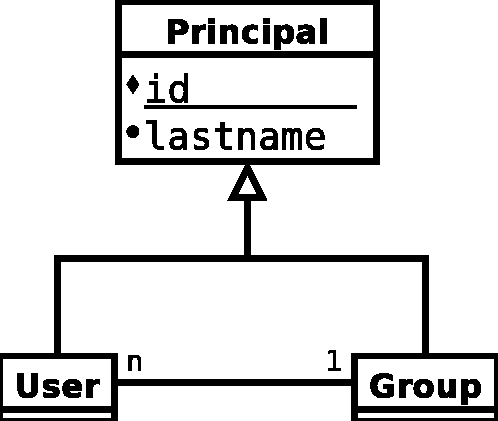
\includegraphics[width=0.4\textwidth]{group-er1.pdf}
\caption{Vztah modelů Principal, User a Group}
\end{figure}

Model Principal se používá v~případech, kdy nezáleží na tom, zda pracujeme
s~uživateli či skupinami, například při přidávání členů projektu.

Přidáním uživatele (skupiny) do projektu vzniká člen (Member). Každý
člen projektu může mít více rolí; dekompozicí této relace je model
\mbox{MemberRole}.

\begin{figure}[htbp]
\centering
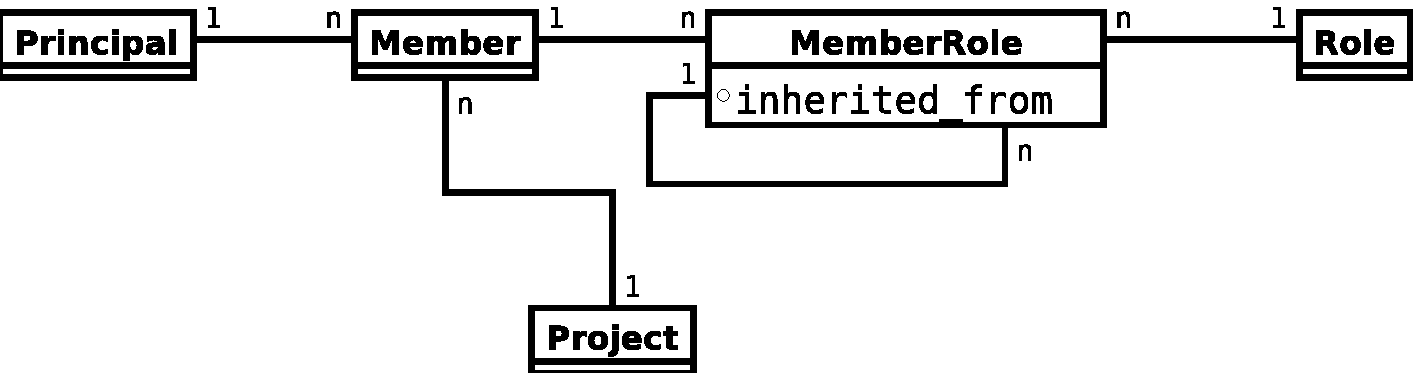
\includegraphics[width=1\textwidth]{group-er2.pdf}
\caption{Vztah uživatelů, rolí a projektů}
\end{figure}

Při přidání skupiny do projektu se reálně přidají členové skupiny jako
členové projektu. ChiliProject mezi takto \uv{zděděnými} uživateli a
individuálně přidanými uživateli rozlišuje na úrovni modelu MemberRole
prostřednictvím atributu \lstinline!inherited_from!, který odkazuje na
původní záznam MemberRole skupiny. Tento model nevypadá příliš
elegantně, ale na druhou stranu tím, že je dědičnost určená pro každou
členskou roli, je pak možné řešit i poměrně složité situace. Například
když je do projektu přidán tentýž uživatel jednou přímo a podruhé v~rámci
skupiny. V~tomto systému si zachová jak svou původní roli, tak zdědí roli
skupiny. Pokud bude skupina z~projektu později odebrána, uživatel
přijde pouze o~svou roli. Pokud člen nemá v~projektu žádnou roli, je jeho
záznam po odebírání poslední role odstraněn.

\subsection{Model projektové skupiny}

Co potřebujeme je speciální typ skupiny, která bude vázaná na konkrétní
projekt. K~tomu lze využít dědičnost, nový model ProjectGroup je
podtřídou modelu Group. Zároveň patří (belongs to) rodičovskému projektu
(asociace \lstinline!parent_project!, model Project).

\begin{figure}[bp]
\centering
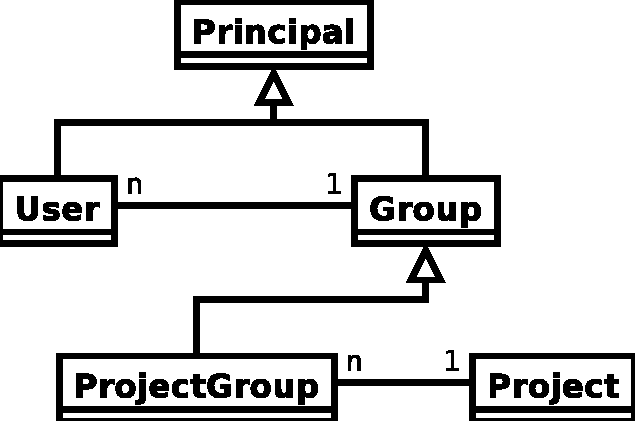
\includegraphics[width=0.4\textwidth]{group-er3.pdf}
\caption{Model ProjectGroup}
\end{figure}

Díky dědičnosti nemusí rozšíření řešit přidávání a správu členství
v~projektech -- o~to se postará standardní implementace třídy Group a
polymorfismus.

Model Project v~tomto vztahu má mnoho (has many) projektových skupin.
Také je zde nutné upravit asociaci \lstinline!member_principals! která
představuje všechny uživatele a skupiny, jenž jsou členy daného projektu.
ChiliProject zde vybírá konkrétní typy záznamů prostřednictvím sloupce
\lstinline!type! -- do podmínky je proto nutné zahrnout i typ
ProjectGroup.

\begin{lstlisting}
# module ProjectGroupPlugin::ProjectPatch
has_many :member_principals, :class_name => 'Member',
:include => :principal,
:conditions => "#{Principal.table_name}.type='ProjectGroup' OR #{Principal.table_name}.type='Group' OR (#{Principal.table_name}.type='User' AND #{Principal.table_name}.status=#{User::STATUS_ACTIVE})"
\end{lstlisting}
Vícenásobné volání makra \lstinline!has_many! nahradí předchozí
definici, proto bude asociace definovaná v~rozšíření brána v~potaz.

Větší problém je s~validátory, které se řetězí -- vícenásobná definice
validace na stejný atribut pouze přidá další \gls{callback} na konec
seznamu validací. To však vadí, pokud chceme z~rozšíření nastavit méně
přísné podmínky platnosti záznamu -- v~tomto případě se jedná
o~unikátnost názvu skupiny. Standardně musí mít každá skupina unikátní
název; u~projektové skupiny však stačí, aby její název byl unikátní pouze v~rámci daného
projektu. Naštěstí jsem nebyl první, kdo podobný problém řešil
\citep{McAlpin2011} -- výsledek není moc pěkný, ale je ukázkou síly
metaprogramování v~Ruby.

Na model Group se při inicializaci aplikuje toto volání:

\begin{lstlisting}
# module ProjectGroupPlugin::GroupPatch
@validate_callbacks.reject! do |c|
  begin
    if Proc === c.method && eval("attrs", c.method.binding).first == :lastname && c.options[:case_sensitive] == false
      true
    end
  rescue
    false
  end
end
\end{lstlisting}
Z~třídní proměnné \lstinline!validate_callbacks! se odstraní ta validace
pro atribut \lstinline!lastname!, která má možnost
\lstinline!case_sensitive! nastavenou na \lstinline!false! -- pokud je pro
tento atribut definováno více validací, poslední kontrola zaručuje, že
se odstraní pouze kontrola unikátnosti (jiné validace s~volbou
\lstinline!case_sensitive! nepracují). Následně se definuje nová
validace omezená na konkrétní projekt; globální skupiny nemají projekt
určený, a tím pádem se budou také validovat se stejným omezením -- je tak
zachována podmínka unikátnosti názvů globálních skupin.

\subsubsection{Dědění skupin v~hierarchii projektů}
\label{sec:proj_group_inherit}

Pro splnění požadavku dědění skupin do podprojektů se nabízí dvě
řešení. Buď se bude relace mezi skupinami a podprojekty udržovat
v~databázi, nebo se zděděné skupiny určí spojením projektů se skupinami a
určí se z~hierarchie projektů.

První možnost je jednodušší z~hlediska Rails a potenciálně nabízí více
možností, například pokud by se projektové skupiny dědily mimo
hierarchii podprojektů nebo by měly mít v~rámci různých projektů různé
vlastnosti. Nevýhodou je pak riziko vzniku nekonzistence v~důsledku
jisté duplikace dat a náročnost některých operací -- při manipulaci
s~projekty či projektovými skupinami (např. přesun projektu, vytvoření
nového projektu či skupiny) se musí udržovat vazby v~hierarchii
podprojektů.

Druhá možnost je čistší z~hlediska databáze, informace o~dědičnosti jsou
na jediném místě.

Pro demonstraci jsem se rozhodl implementovat obě řešení v~rámci dvou
rozšíření -- skupiny používají první možnost, role používají možnost
druhou.

Mezi modely ProjectRole a Project vznikne nová M:N vazba, tu jsem
dekomponoval do modelu ProjectGroupScope (konvence ActiveRecord nabízela
název ProjectGroupProject, což mi nepřišlo moc rozumné).

\begin{figure}[htbp]
\centering
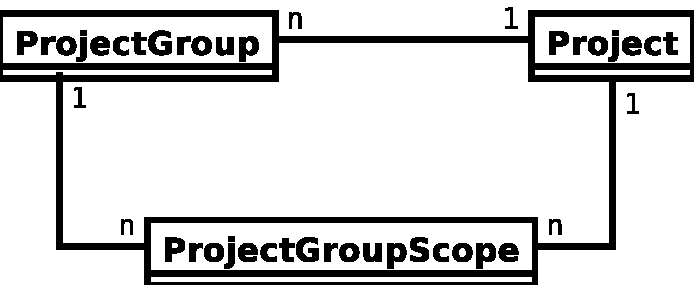
\includegraphics[width=0.5\textwidth]{group-er4.pdf}
\caption{Vazba ProjectGroup--ProjectGroupScope--Project}
\end{figure}

Projektové skupiny se budou vždy vybírat přes tuto vazbu, budou zde
proto zahrnuty i vazby mezi rodičovskými projekty a jejich vlastními
potomky.

Pro udržování vazeb lze použít zpětná volání ActiveRecord -- konkrétně
když je projektová skupina vytvořena, musí se propagovat do podprojektů
rodičovského projektu -- k~tomu poslouží zpětné volání
\lstinline!after_create!, ve kterém skupina vytvoří vazby na následníky
projektu. Při odstranění skupiny se vazby odstraní automaticky.

Zvláštní případ je však přesun projektu. Zde se nejedná o~zpětné volání
ActiveRecord, ale o~metodu \lstinline"set_parent!" v~ChiliProjectu,
která se volá při každé změně hierarchie. V~takovém případě se přebudují
vazby pro přesunutý projekt a jeho potomky (projekt lze přesunout pouze
jako celek se všemi potomky, nikoliv však do svého podstromu). Přesunutý
projekt nahradí původní zděděné skupiny skupinami svého rodiče, a to se
rekurzivně opakuje až k~listům.
Tato operace se provede i při vytvoření nového projektu, nejvýše však
jednou; nový projekt nemůže mít žádného potomka.

\subsection{Manipulace se skupinami, autorizace}

Aby bylo možné projektové skupiny spravovat, je pro ně nutné vytvořit
administrační rozhraní. Zde lze vyjít ze standardní správy skupin, kterou
ChiliProject obsahuje.

\begin{figure}[tbp]
\centering
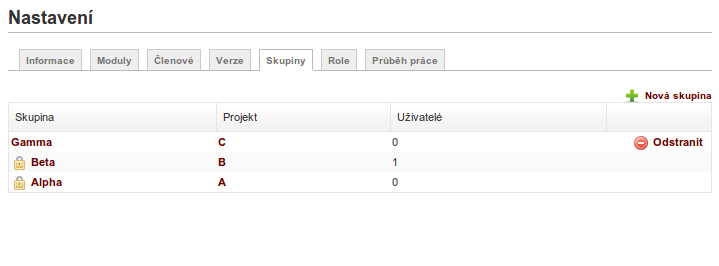
\includegraphics[width=1\textwidth]{group-gui1.png}
\caption{Správa projektových skupin}
\end{figure}

Správa skupin je umístěná v~nastavení projektu -- zde je možné prohlížet
projektové skupiny, které má daný projekt k~dispozici, a vytvářet nové.
Patří-li skupina tomuto projektu, je možné ji upravovat (přidávat
uživatele, měnit název). Pokud ne, může si správce pouze zobrazit seznam
členů této skupiny.

Na záložce Členové, v~nastavení projektu, se projektové skupiny zobrazí
stejně jako globální skupiny a je možné mezi nimi vyhledávat. K~tomu
však bylo nutné nahradit odpovídající pohled
\lstinline!projects/settings/members! -- protože totéž bylo nutné
později provést i pro projektové role, vyextrahoval jsem tento pohled do
samostatného rozšíření \emph{Members View},
které funguje také jako \gls{gem}.

Z~hlediska autorizace přidává rozšíření jedno oprávnění: \emph{Manage
project groups} -- má-li uživatel roli s~tímto oprávněním (společně
s~možností spravovat projekt), bude moct pracovat se skupinami v~daném
projektu. K~oprávnění se vážou specifické akce controlleru
ProjectGroupsController, kde se navíc kontroluje, zda daná skupina patří
projektu a je ji tím pádem možné měnit.

\subsection{Testy}

Testy pokrývají především funkčnost controllerů (včetně autorizace),
patchů a složitějších operací s~modely, jako je například zmíněná změna
hierarchie projektů.

Dochází zde k~určitému překryvu mezi funkcionálními a jednotkovými testy, nicméně
jsem se snažil klást důraz na funkcionální testy, které lépe vystihují
konečné chování rozšíření.

Pouze jedna chyba se projevila až při nasazení na produkční server:
administrace globálních skupin fungovala do té doby, než uživatel jednou
otevřel správu projektových skupin. Systém se v~administraci globálních
skupin nepokoušel načíst z~databáze projektové skupiny, pokud jejich
třída nebyla předtím použita. To je důsledek cachování tříd, ovšem tato funkce je
ve vývojovém režimu Rails vypnutá, aby nebylo nutné restartovat
aplikační server při každé změně kódu\footnote{Novější verze Rails navíc
  detekují změny v~souborech a obnovují jen ty třídy, které byly
  změněny.}.

\subsection{Zhodnocení}

Rozšíření splňuje všechny požadavky a bylo otestováno jak automatickými
testy, tak manuálně. Jedna z~funkcí, která by mohla být v~budoucnu
implementována, je kopírování skupin, což by bylo užitečné zejména
v~kontextu projektových skupin (mohu si zkopírovat zděděnou skupinu do
svého projektu a dále ji upravovat).

\section[Správa rolí a workflow na úrovni projektů]{Správa rolí a workflow na úrovni projektů (ChiliProject Project
Roles)}
\label{sec:project_roles}

\subsection{Specifikace}

Cíl tohoto rozšíření je podobný jako u~projektových skupin -- poskytnout
správcům projektů více možností a více decentralizovat správu. Toto
rozšíření však může mít mnohem větší dopad na práci se systémem
ChiliProject.

Uživatel s~oprávněním pro modifikaci projektových rolí může:

\begin{enumerate}[1.]
\item
  Vytvářet či mazat projektové role (v~kontextu daného projektu),
\item
  upravovat práva projektových rolí,
\item
  změnit práva role anonymous či non-member v~kontextu projektu.
\end{enumerate}
Kromě rolí definovaných administrátorem má ChiliProject navíc dvě
vestavěné role: \emph{anonymous} (pro nepřihlášeného uživatele) a
\emph{non-member} (pro uživatele, který v~kontextu projektu není jeho
členem).

S~funkcemi rolí je úzce spjatý systém \gls{workflow} -- pokud by tato
funkce nebyla zahrnuta, projektové role by mohly používat
issue tracker pouze omezeně.

Uživatel s~oprávněním pro modifikaci projektového \gls{workflow} může:

\begin{enumerate}[1.]
\setcounter{enumi}{3}
\item
  Měnit a kopírovat workflow pro projektové role.
\end{enumerate}
\subsection{Existující řešení}

Část požadovaných funkcí nabízí rozšíření Role Shift\footnote{\url{http://projects.andriylesyuk.com/projects/role-shift}},
které funguje na principu \emph{posunu} role -- jedna role se tak
v~určitém projektu může chovat jako jiná. Ačkoli to nezní moc užitečně,
částečně to řeší požadavek 3, protože je tím možné předefinovat i vestavěné
role. Právě pro řešení vestavěných rolí se tato strategie ukázala jako
nejschůdnější.

\subsection{Systém rolí a oprávnění}

Jaký je vztah rolí vůči uživatelům a projektům už jsem naznačil
(\ref{sec:proj_group_sys}). Oprávnění nemají v~systému samostatný model,
většinou se s~nimi pracuje na úrovni rolí jako s~polem symbolů.

Pokud je zapotřebí zajistit autorizaci uživatele, použije se instanční
metoda \lstinline!Principal#allowed_to?! která dostane symbol
představující určité oprávnění (například
\lstinline!:manage_project_roles!), kontext (tím může být projekt, pole
projektů, nebo \lstinline!nil!) a volbu, zda se má kontrolovat globální
kontext -- ten se používá například u~vytváření nových projektů, které
nemají rodiče, tj. tam, kde nelze vyjít z~kontextu existujícího
projektu. Pro ověření autorizace se projdou všechny role, které daný
uživatel má v~daném kontextu -- projektu (či v~projektech). Pokud se
u~nějaké role najde hledané oprávnění, je autorizace úspěšná.

\subsubsection{Model projektových rolí}

Obdobně jako u~projektových skupin je projektová role (LocalRole)
podtřídou standardního modelu Role a přidává vazbu na rodičovský
projekt.

\begin{figure}[htbp]
\centering
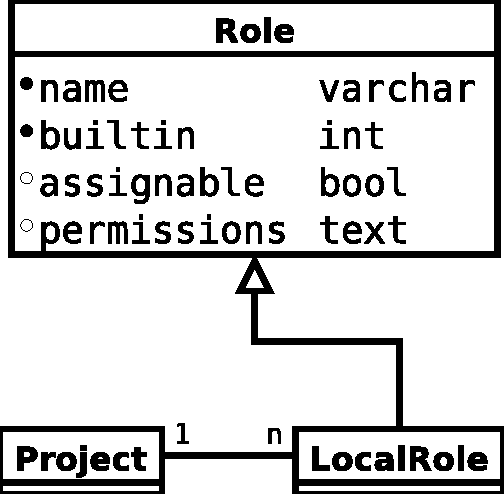
\includegraphics[width=0.4\textwidth]{role-er1.pdf}
\caption{Model LocalRole}
\end{figure}

Projektová role se z~hlediska autorizace chová stejně jako normální
role, s~výjimkou autorizace v~globálním kontextu -- v~takovém případě
nesmí být projektové role brány v~potaz a z~kontroly práv jsou zcela
vyloučeny. V~kontextu projektu se pak kontrolují pouze ty role, které má
uživatel v~tomto projektu přiřazené, není zde tedy nutné dodatečně
kontrolovat, zda prověřovaná role do projektu skutečně patří. Nicméně
tato kontrola je prováděná u~člena projektu (model Member), kde validace
zabrání vzniku členství s~rolemi, které nepatří do hierarchie projektu.

Pro dědění rolí do podprojektů jsem z~popsaných možností
(\ref{sec:proj_group_inherit}) použil druhou variantu. Jádrem tohoto
řešení je \gls{scope} v~modelu Role, který vybere projektové role
z~předchůdců rodičovského projektu společně s~globálními rolemi:

\begin{lstlisting}
named_scope :available_for_project, lambda { |project|
{:joins => "LEFT OUTER JOIN projects ON roles.local_role_project_id = projects.id",
 :conditions => ["roles.type = 'Role' OR (roles.type = 'LocalRole' AND projects.lft <= ? AND projects.rgt >= ?)", project.left, project.right] }
}
\end{lstlisting}
Obdobné řešení lze použít, pokud takto chceme vybrat pouze lokální role.

Tímto lze vyřešit vytváření a aplikování projektových rolí, jak si však
poradit se speciálními rolemi?

\subsubsection{Posun rolí}

Uvažoval jsem nad různými variantami, jak v~rozšíření zpracovat speciální
role \emph{non-member} a \emph{anonymous}. Většina návrhů měla problém
s~děděním rolí. Nebylo možné je vyřešit dostatečně transparentně a
přívětivě pro správce projektu, nebo narážela na prostý fakt, že
ChiliProject počítá s~tím, že v~databázi existuje pouze jediná speciální
role daného druhu. Nakonec jsem použil modifikaci řešení od Andriye
Lesyuka ze zmíněného rozšíření Role Shift.

Do aplikace je přidán nový model RoleShift, který je dekompozicí M:N
relace mezi projektem a rolí.

\begin{figure}[htbp]
\centering
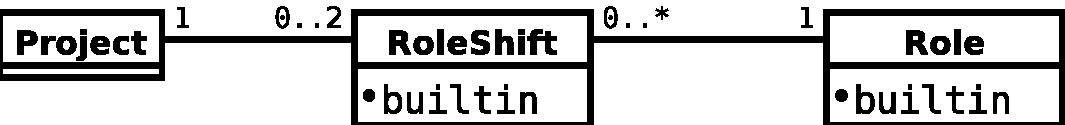
\includegraphics[width=1\textwidth]{role-er2.pdf}
\caption{Model RoleShift}
\end{figure}

Každý projekt může mít nejvýše dva záznamy RoleShift:
\lstinline!role_non_member! a \lstinline!role_anonymous! (typ je určený
pomocí atributu \lstinline!builtin!). Pokud tyto záznamy existují, budou
s~nimi asociované role použity namísto odpovídajících globálních rolí.

Správce tak má pod kontrolou, zda chce výchozí globální roli nahradit či
nikoliv, navíc je možné použít jednotnou správu projektových rolí a
jejich dědičnost.

\subsubsection{Manipulace s~projektovými rolemi}

Pro controller a pohledy bylo opět možné vyjít ze standardní správy
rolí.

\begin{figure}[tbp]
\centering
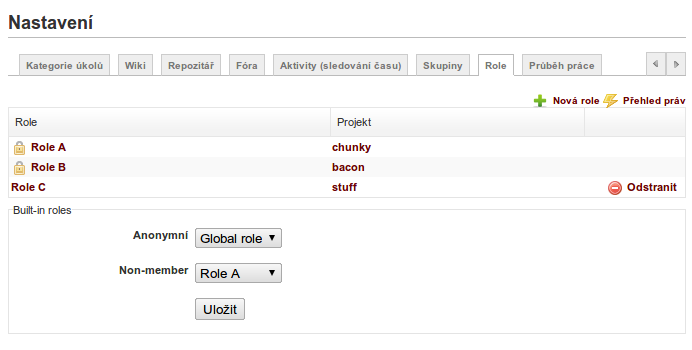
\includegraphics[width=1\textwidth]{role-gui1.png}
\caption{Správa projektových rolí}
\end{figure}

Autorizace je rozdělená do dvou oprávnění -- \emph{Manage project roles} a
\emph{Manage role shifts}. Důvodem je, že o~projektové role a o~posuny rolí
se starají dva různé controllery a ChiliProject nenabízí způsob, jak
sloučit autorizaci k~více controllerům pod jediné oprávnění. Návrh však
předpokládá, že tato dvě oprávnění budou používaná společně.

\subsection{Správa workflow}

V~případě \gls{workflow} není nutné přidávat další modely -- je možné
využít standardní asociace s~modelem Role.

\begin{figure}[htbp]
\centering
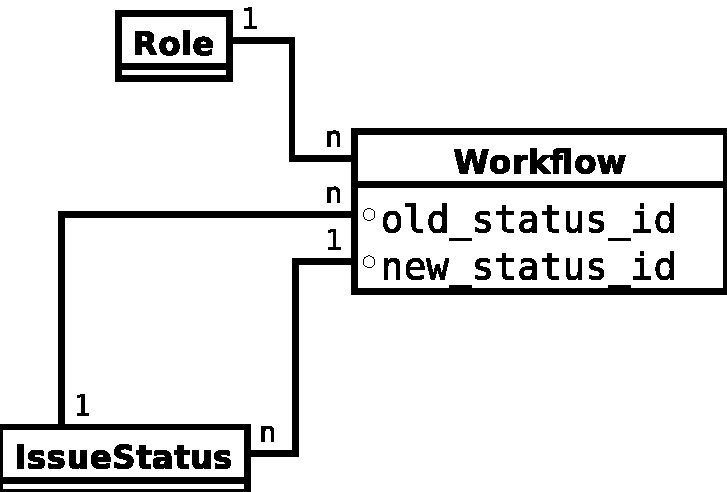
\includegraphics[width=0.5\textwidth]{role-er3.pdf}
\caption{Vazby Workflow}
\label{fig:Workflow}
\end{figure}

V~rámci rozšíření tak stačí zajistit možnost správy workflow ve vlastním
controlleru (LocalWorkflowsController). Ten je téměř stejný jako
standardní controller (WorkflowsController), rozdíl je však v~rozsahu
rolí, se kterými pracuje. V~rámci projektu je možné editovat pouze
workflow těch rolí, které bezprostředně patří danému projektu.

I~workflow mají samostatné oprávnění \emph{Manage project workflows}.

\subsection{Testy}

Logika testů pro práci s~rolemi a workflow byla velice podobná
standardním testům odpovídajících funkcí v~ChiliProject, nicméně jsem
testy přepsal do konvencí Shoulda a rozšířil je o~kontrolu autorizace a
dalších omezení.

\subsection{Zhodnocení}

Požadavky byly splněny a funkčnost rozšíření byla otestována. Podobně
jako u~projektových skupin se pro další vývoj
nabízí implementace kopírování rolí.

Nabízí se zde také jistý prostor pro optimalizaci dotazování databáze -- zejména
posun rolí se provádí při téměř každé akci bez ohledu na to, zda nějaká
náhradní role existuje -- to však vyžaduje podrobnější určení
\glspl{scope} vhodných pro optimalizaci.

Vzhledem ke komplexitě a množství metod, které rozšíření nahrazuje
v~jádru aplikace, může dojít ke konfliktům s~jinými rozšířeními. Takové
případy však bude nutné řešit individuálně úpravou tohoto nebo
konfliktního rozšíření.

\section[Wiki stránky s~omezeným přístupem]{Wiki stránky s~omezeným přístupem (ChiliProject Private
Wiki)}
\label{sec:private_wiki}

\subsection{Specifikace}

Rozšíření by mělo umožnit vytváření soukromých stránek na \gls{wiki},
které budou přístupné pouze uživatelům s~odpovídajícím oprávněním. Zcela
původní návrh hovořil o~komplexní správě přes \gls{ACL} s~individuální
správou konkrétních akcí (prohlížení, úprava, přístup k~historii atp.),
ale nakonec bylo upřednostněno jednodušší řešení. Mimo jiné s~ohledem k~tomu, že
správa projektových rolí může tyto funkce celkem dobře nahradit. Role
však pracují s~wiki v~projektu jako celkem, proto toto rozšíření umožňuje
jemnější řízení přístupu ke konkrétním stránkám. Rozšíření by mělo
respektovat hierarchii stránek -- pokud je soukromý některý
z~předchůdců, bude daná stránka také soukromá.

Uživatelé budou moct získat dvě nová oprávnění: správa viditelnosti
stránky a přístup na soukromé stránky. První oprávnění dává uživateli
možnost nastavit stránku jako soukromou, druhé umožňuje aby vůbec mohl
vidět obsah stránky.

\subsection{Existující řešení}

V~tomto případě už existuje poměrně funkční řešení v~podobě rozšíření
Redmine Private Wiki\footnote{\url{https://github.com/f0y/redmine_private_wiki}},
které napsal Oleg Kandurov. Autor ovšem nespecifikoval licenci. Po
ujištění, že je kód dostupný pod permisivní MIT licencí (která byla
zachována), jsem vytvořil \gls{fork} rozšíření, obligátně nazvaný
ChiliProject Private Wiki.

\subsection{Úprava rozšíření Private Wiki}

Rozšíření přidává k~wiki stránkám dodatečný booleovský atribut
\lstinline!private!. Pro zajištění dodatečné autorizace se provede
\lstinline!before_filter! v~controlleru wiki stránek
(WikiPagesController), který po standardní autorizace zkontroluje, zda je
stránka soukromá a zda daný uživatel má oprávnění k~ní přistupovat. Mimo
to zajišťuje rozšíření změnu atributu \lstinline!private!
prostřednictvím nové akce v~controlleru -- tu může oprávněný uživatel
vyvolat prostřednictvím odkazu na wiki stránce. Uživatelské rozhraní je
upraveno pomocí JavaScriptu -- pohledy bohužel nemají dostatek zpětných
volání, aby je bylo možné rozšířit na straně serveru. O~přístupnosti pro
uživatele s~vypnutým JavaScriptem však beztak nelze hovořit, protože
samotný framework Rails vyžaduje JavaScript i pro běžnou uživatelskou
interakci\footnote{Rails 3 používá \uv{unobtrusive JavaScript}
  což tento problém z~velké části řeší.}.

\begin{figure}[tbp]
\centering
\centerline{
\includegraphics[width=1.2\textwidth]{wiki-gui1.png}}
\caption{Soukromá stránka na wiki}
\label{fig:GUIPrivateWiki}
\end{figure}

Rozšíření má však některé nedostatky -- nerespektuje hierarchii stránek
a nemá testy.

Na rozdíl od projektů je hierarchie wiki stránek v~databázi řešena jako
jednoduchý strom, kdy stránka odkazuje pouze na svého bezprostředního
rodiče přes sloupec \lstinline!parent_id!. Při procházení ke kořeni se
pro každého předka provede nový dotaz do databáze -- na druhou stranu,
Rails v~rámci jedné akce implicitně cachuje výsledky totožných dotazů,
tudíž se tato operace provede pouze jednou. Kontrola soukromých stránek
v~rámci hierarchie bude mít na výkon aplikace jen minimální dopad --
ChiliProject beztak vypisuje seznam předků stránky (tzv. drobečková
navigace), takže databáze dostane tuto sadu dotazů i bez tohoto
rozšíření.

V~tomto případě, vzhledem k~tomu, že jde o~rozšíření, které zpřísňuje
autorizaci, jsou nejdůležitější funkcionální testy controlleru. Použil
jsem zde (podobně jako u~ostatních rozšíření) hromadný test, zda soukromá
stránka zablokuje všechny akce pro neautorizovaného uživatele:

\begin{lstlisting}
{:rename => :get, :edit => :get, :update => :put, :protect => :post, :history => :get,
 :diff => :get, :annotate => :get, :add_attachment => :post, :destroy => :delete}.each do |action, verb|
  context "#{verb.to_s.upcase} #{action}" do
    setup do
      self.send verb, action, :project_id => @project, :id => @page.title
    end
    should_respond_with 403 # access denied
  end
end
\end{lstlisting}
Tento fragment vytvoří devět testů pro různé akce s~příslušnými metodami
a očekává, že ve všech případech controller vrátí HTTP kód 403
(přístup zakázán). Není to samozřejmě neprůstřelná metoda; pokud do
controlleru přibude nová akce, je nutné test aktualizovat -- zde by bylo
zajímavé využití reflexe pro automatické určení metod pro testování.

\subsection{Zhodnocení}

Toto rozšíření je poměrně jednoduché jak z~vývojářského, tak
z~uživatelského hlediska. Zajímavé bude sledovat jeho využívání
v~praxi -- v~kombinaci s~projektovými rolemi se jedná
o~zajímavou alternativu k~plnohodnotnému \gls{ACL}, která jen minimálně
zatěžuje uživatele.

Další vývoj by mohl například přidat přehled soukromých stránek a
případně jejich hromadnou správu. Užitečná by byla i možnost přímého vytvoření
soukromé stránky -- volba by byla dostupná hned ve formuláři.

\section[Úkoly s~omezeným přístupem]{Úkoly s~omezeným přístupem (ChiliProject Private Issues)}
\label{sec:private_issues}

\subsection{Specifikace}

Cíl je podobný jako u~soukromých wiki stránek -- některé úkoly v~issue
trackeru budou označené jako soukromé, a uvidí je pouze oprávnění
uživatelé. Jsou zde však jistá specifika; uživatel by měl vidět úkol,
který sám vytvořil, nebo mu byl přiřazen, a to bez ohledu na to,
zda má příslušné oprávnění, nebo ne.

Opět jsou zde dvě oprávnění: nastavení viditelnosti úkolu a přístup
k~soukromým úkolům. Uživatel má přístup k~soukromému úkolu, pouze pokud má
příslušné oprávnění, je autorem úkolu a nebo byl k~němu přiřazen --
obdobně jako s~přístupem je to i s~viditelností úkolu v~přehledu úkolů.

\subsection{Existující řešení}
\label{sec:private_issues_exist}

V~této oblasti je Redmine napřed -- viditelnost úkolů je možné určit od
verze 1.2\footnote{\url{http://www.redmine.org/issues/7414}}.
ChiliProject tuto funkci neimplementoval s~odvoláním na to, že systém
oprávnění bude beztak zapotřebí kompletně přepracovat,\footnote{\url{https://www.chiliproject.org/issues/189}}
bohužel se tato iniciativa zatím nedostala moc daleko. Implementace
v~Redmine alespoň může posloužit jako reference pro samostatné
rozšíření.

\subsection{Implementace rozšíření}

Základní idea je stejná jako u~wiki stránek -- controller zakáže přístup,
pokud uživatel neprojde autorizací. Oříškem je však rozhraní pro
vybírání úkolů z~databáze -- model Query. Kromě jednoduchého výpisu
úkolů umožňuje i předdefinovat specifické kombinace dotazů. Uvnitř se
jedná o~velký generátor SQL, který občas může vrátit klauzuli
\lstinline!WHERE 0=1!. Rozšíření nemá mnoho možností, jak ovlivnit
generování dotazu. Jedině odchytit vygenerovaný řetězec
s~dotazem a připojit k~němu vlastní podmínky:

\begin{lstlisting}
# module PrivateIssues::QueryPatch
def statement_with_private_issues
  filters_clauses = statement_without_private_issues

  user = User.current
  unless project && user.allowed_to?(:view_private_issues, project)
    filters_clauses << " AND (issues.private = #{connection.quoted_false} OR issues.author_id = #{user.id} OR issues.assigned_to_id = #{user.id})"
  end
  filters_clauses
end
\end{lstlisting}
Testy pak kontrolují, zda se úkol zobrazí ve výpisu uživateli
s~oprávněním pro prohlížení soukromých úkolů, stejně tak i pro uživatele,
který je k~úkolu přiřazený. Obdobně je tomu i s~přístupností
controlleru.

\begin{figure}[tbp]
\centering
\centerline{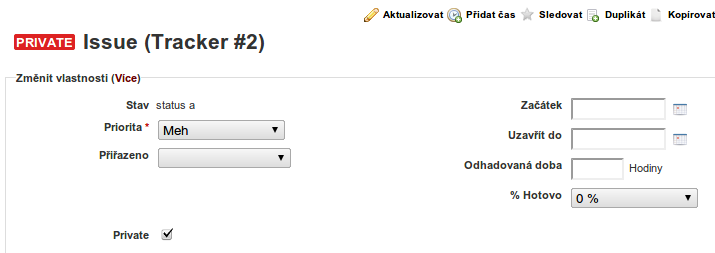
\includegraphics[width=1.2\textwidth]{issues-gui1.png}}
\caption{Soukromý úkol}
\end{figure}

\subsection{Zhodnocení}

Tato implementace sice není tak funkční jako vestavěná funkcionalita
v~Redmine, nicméně svoji úlohu plní. V~budoucích verzích by zřejmě bylo
dobré rozdělit přidružená oprávnění, což by umožnilo podrobněji
definovat, co uživatelé mohou, a co ne. Bylo by možné také hlouběji
propracovat integraci s~vyhledáváním úkolů -- mohlo by se jednat
o~kritérium, což by umožnilo snadno nalézt všechny soukromé úkoly.

\section[Přidávání uživatelů z~LDAP]{Přidávání uživatelů z~LDAP (ChiliProject Add LDAP Users)}
\label{sec:add_ldap_users}

\subsection{Požadavky}

Pro přidání uživatele do systému ChiliProject je nutné projít
registrační procedurou -- vyplnit jméno, heslo, e-mail\ldots{} Přitom
všechny tyto údaje jsou k~dispozici přes \gls{LDAP}, který systém již
umí používat. I~když se uživatel poprvé přihlásí s~údaji z~\gls{LDAP},
je mu automaticky vytvořen účet bez nutnosti cokoliv vyplňovat. Je tedy
celkem logické, aby existovala funkce, která umožní administrátorovi
importovat uživatele zadáním uživatelského jména.

Rozšíření přidá novou stránku do administrace, kde je možné zadat
uživatelská jména -- pokud je takto nalezen uživatel, který doposud není
v~databázi ChiliProjectu, bude mu automaticky vytvořen účet, stejně jako
by se zaregistroval.

\subsection{Implementace rozšíření}

Autentizace uživatelů je řešena přes abstraktní model AuthSource.
ChiliProject standardně obsahuje autentizaci přes \gls{LDAP} -- model
AuthSourceLdap. Z~toho je zřejmé, že autentizace je modulární; lze
snadno definovat nové autentizační zdroje a použít je v~projektu, přičemž
postačí, když budou dodržovat definované rozhraní.

Toto rozšíření však pracuje s~modelem AuthSourceLdap. Ten umí
autentizovat uživatele dle zadané dvojice jméno-heslo a vrátit údaje pro
další zpracování. Nejprve z~adresáře stáhne údaje o~uživateli, čímž
také ověří, že vůbec existuje
(\lstinline!AuthSourceLdap#get_user_dn!), následně se pokusí s~předanými
údaji k~adresáři připojit. V~rozšíření potřebujeme provést pouze první
část -- získat z~adresáře údaje o~uživateli -- a následně vytvořit
záznam uživatele. Patch pro AuthSourceLdap přidává metodu
\lstinline!get_user!, se kterou pak pracuje samostatný controller
\lstinline!LdapUsersController! dostupný přes administraci.

Součástí rozšíření nejsou testy -- v~praxi se ukázalo jednodušší
vyzkoušet funkčnost s~fakultním LDAP serverem, než server simulovat.
Pravděpodobně by ani testy nepomohly objevit problém s~kódováním řetězců
získaných přes LDAP. Vypsání těchto řetězců (typicky se jednalo o~plné
jméno přidávaného uživatele) způsobilo chybu ve vykreslování stránky.
Mock server by tuto chybu neodhalil.

\subsection{Zhodnocení}

Toto rozšíření je velice jednoduché a považuji jej spíš za funkční
prototyp, který by se mohl stát součástí rozsáhlejší integrace služeb
LDAP serveru. Při přidávání uživatelů by ChiliProject mohl, například
při přidávání uživatele do projektu, \uv{našeptávat} uživatele nalezené
v~adresáři podle zadaných údajů, a následně jim vytvořit účty -- částečně
by se tak smazala hranice mezi lokální databází a externími zdroji.

Jako minimální implementace však může sloužit toto rozšíření už nyní.

\begin{conclusion}

Cílem práce bylo analyzovat a zvolit nejvhodnější řešení pro správu projektů v~Oddělení ICT Fakulty informačních technologií. Pro vybraný systém pak byla implementována rozšíření, která ho dále přizpůsobila potřebám oddělení. Funkčnost rozšíření byla otestována manuálně i prostřednictvím automatických testů, dále byla ověřena vzájemná nekonfliktnost a integrace všech rozšíření -- systém jako celek prošel všemi automatickými testy. Z~tohoto hlediska lze práci hodnotit jako úspěšnou.

Mým cílem bylo implementovat veškeré přidané funkce jako rozšíření, bez zásahu do jádra aplikace -- tento cíl se mi také podařilo splnit a věřím, že to bude mít pozitivní vliv jak pro ICT oddělení v~podobě snadnější správy aktualizací, tak pro budoucí vývoj jednotlivých rozšíření, která mohou být zapojena do komunitního vývoje.

Rozšíření jsou v~současnosti provozována na testovacím serveru; nepředpokládám, že nový systém bude ihned uveden do provozu, bude vhodné jej nejprve otestovat s~reálnými uživateli a daty. Jako jedno z~řešení pro postupnou migraci se nabízí provoz testovacího serveru nad replikou databáze současného systému. Testovací provoz je i vhodnou příležitostí pro nasazení moderního software, ať už je to Ruby 1.9.3 či poslední generace aplikačního serveru Passenger \citep{Passenger32}.

Modifikace uvedené v~této práci představují pouhý zlomek funkcí, které mohou dále zjednodušit správu projektů a zlepšit uživatelský komfort.

\end{conclusion}

\bibliographystyle{csn690}
\bibliography{ref}

\appendix

\glsaddall
\printglossaries

\chapter{Seznam systémů uvažovaných pro hodnocení}
\label{chap:seznampm}

\begin{description}
\item[Trac] \url{http://trac.edgewall.org/}
\item[The Bug Genie] \url{http://www.thebuggenie.com/}
\item[Teambox] \url{http://www.teambox.com/}
\item[Launchpad] \url{https://dev.launchpad.net/}
\item[Open Atritum] \url{http://openatrium.com/}
\item[Redmine] \url{http://www.redmine.org/}
\item[ChiliProject] \url{https://www.chiliproject.org/}
\item[GitLab] \url{http://gitlabhq.com/}
\item[Collabtive] \url{http://collabtive.o-dyn.de/}
\item[mtrack] \url{http://mtrack.wezfurlong.org/}
\item[GLPI] \url{http://www.glpi-project.org/spip.php?lang=en}
\item[Request Tracker] \url{http://bestpractical.com/rt/}
\item[OTRS Help Desk] \url{http://www.otrs.com/en/products/otrs-help-desk/}
\item[Roundup] \url{http://www.roundup-tracker.org/}
\item[LibreSource] \url{http://dev.libresource.org/ (Kompletní groupware včetně integrace s~Jabberem -> overkill?)}
\item[PHProjekt] \url{http://www.phprojekt.com/ (sami používají JIRA+Confluence)}
\item[TeamLab] \url{http://www.teamlab.com/ (GPLv3 – http://sourceforge.net/projects/teamlab/)}
\item[Retrospectiva] \url{https://github.com/dim/retrospectiva}
\item[Plancake] \url{http://www.plancake.com/}
\item[Project HQ] \url{http://projecthq.org/}
\item[Streber PM] \url{http://www.streber-pm.org/}
\item[Project Pier] \url{http://www.projectpier.org/}
\item[Todoyu] \url{http://www.todoyu.com/}
\end{description}

\chapter{Obsah přiloženého média}

U~jednotlivých rozšíření je připojený textový soubor README.md
s~instrukcemi a popisem funkcí.

\begin{figure}
	\dirtree{%
		.1 chiliproject-fit\DTcomment{distribuce ChiliProject včetně rozšíření}.
		.1 plugins\DTcomment{jednotlivá rozšíření}.
		.2 engines\DTcomment{opravená verze Engines}.
		.2 chiliproject\_add\_ldap\_users\DTcomment{přidávání uživatelů z~LDAP}.
		.2 chiliproject\_members\_view\DTcomment{pomocné rozšíření pro sdílené pohledy}.
		.2 chiliproject\_private\_issues\DTcomment{soukromé úkoly}.
		.2 chiliproject\_private\_wiki\DTcomment{soukromé stránky na wiki}.
		.2 chiliproject\_project\_group\DTcomment{projektové skupiny}.
		.2 chiliproject\_project\_roles\DTcomment{projektové role}.
		.2 chiliproject\_test\_plugin\DTcomment{prototyp rozšíření pro testování}.
		.1 text\DTcomment{text práce}.
		.2 src\DTcomment{zdrojová forma práce ve formátu \LaTeX{}}.
		.2 BP\_Vlnas\_Jan\_2012.pdf\DTcomment{text práce ve formátu PDF}.
	}
\end{figure}

\end{document}
